\documentclass[preprint]{imsart}

%% Packages
\RequirePackage{amsthm,amsmath,amsfonts,amssymb}
\RequirePackage[numbers,sort&compress]{natbib}
%\RequirePackage[authoryear]{natbib}%% uncomment this for author-year citations
\RequirePackage[colorlinks,citecolor=blue,urlcolor=blue]{hyperref}
\RequirePackage{graphicx}
\RequirePackage{enumerate}
\RequirePackage{pgf}

\startlocaldefs
%%%%%%%%%%%%%%%%%%%%%%%%%%%%%%%%%%%%%%%%%%%%%%
%%                                          %%
%% Uncomment next line to change            %%
%% the type of equation numbering           %%
%%                                          %%
%%%%%%%%%%%%%%%%%%%%%%%%%%%%%%%%%%%%%%%%%%%%%%
%\numberwithin{equation}{section}
%%%%%%%%%%%%%%%%%%%%%%%%%%%%%%%%%%%%%%%%%%%%%%
%%                                          %%
%% For Axiom, Claim, Corollary, Hypothesis, %%
%% Lemma, Theorem, Proposition              %%
%% use \theoremstyle{plain}                 %%
%%                                          %%
%%%%%%%%%%%%%%%%%%%%%%%%%%%%%%%%%%%%%%%%%%%%%%
\theoremstyle{plain}
\newtheorem{axiom}{Axiom}
\newtheorem{claim}[axiom]{Claim}
\newtheorem{theorem}{Theorem}[section]
\newtheorem{lemma}[theorem]{Lemma}
%%%%%%%%%%%%%%%%%%%%%%%%%%%%%%%%%%%%%%%%%%%%%%
%%                                          %%
%% For Assumption, Definition, Example,     %%
%% Notation, Property, Remark, Fact         %%
%% use \theoremstyle{definition}            %%
%%                                          %%
%%%%%%%%%%%%%%%%%%%%%%%%%%%%%%%%%%%%%%%%%%%%%%
\theoremstyle{definition}
\newtheorem{definition}[theorem]{Definition}
\newtheorem*{example}{Example}
\newtheorem*{fact}{Fact}
%%%%%%%%%%%%%%%%%%%%%%%%%%%%%%%%%%%%%%%%%%%%%%
%% Please put your definitions here:        %%
%%%%%%%%%%%%%%%%%%%%%%%%%%%%%%%%%%%%%%%%%%%%%%
\newcommand{\R}{\mathbb{R}}
\newcommand{\N}{\mathbb{N}}
\newcommand{\E}{\mathbb{E}}
\newcommand{\Prob}{\mathbb{P}}
\newcommand{\Var}{\operatorname{Var}}
\newcommand{\Cov}{\operatorname{Cov}}
\newcommand{\KL}{\operatorname{KL}}
\newcommand{\supp}{\operatorname{supp}}
\newcommand{\argmin}{\operatorname*{arg\,min}}
\newcommand{\argmax}{\operatorname*{arg\,max}}
\newcommand{\dd}{\,\mathrm{d}}
\newcommand{\Normal}{\mathcal{N}}
\newcommand{\Emp}{\widehat P_n}
\newcommand{\fhat}{\widehat f}
\newcommand{\Phat}{\widehat P_n}
\newcommand{\phit}{\varphi_t}
\newcommand{\ind}{\mathbf{1}}
\newcommand{\calE}{\mathcal{E}}
\newcommand{\calF}{\mathcal{F}}
\newcommand{\calM}{\mathcal{M}}
\newcommand{\calL}{\mathcal{L}}
\newcommand{\calC}{\mathcal{C}}
\newcommand{\TV}{\operatorname{TV}}
\newcommand{\ISE}{\operatorname{ISE}}
\newcommand{\MISE}{\operatorname{MISE}}
\newcommand{\AMISE}{\operatorname{AMISE}}
\newcommand{\tr}{\operatorname{tr}}
\newcommand{\diag}{\operatorname{diag}}
\newcommand{\Vol}{\operatorname{Vol}}
\newcommand{\rank}{\operatorname{rank}}
\endlocaldefs

\begin{document}

\begin{frontmatter}
\title{Density Evolution: A Multiscale View of Density Estimation}
\runauthor{K. You}
\runtitle{Density Evolution}

\begin{aug}
%%%%%%%%%%%%%%%%%%%%%%%%%%%%%%%%%%%%%%%%%%%%%%%
%% Additional information such as            %%
%% identifying the corresponding author must %%
%% be included in in the Acknowledgments     %%
%% section if necessary.                     %%
%% ORCID can be inserted by command:         %%
%% \orcid{0000-0000-0000-0000}               %%
%%%%%%%%%%%%%%%%%%%%%%%%%%%%%%%%%%%%%%%%%%%%%%%
\author[A,B]{\fnms{Kisung}~\snm{You}}

\address[A]{Department of Mathematics, Baruch College}
\address[B]{Department of Mathematics, The Graduate Center, City University of New York}

%\address[B]{Name2 Surname2 is Professor, Department,University or Company Name, City, Country\printead[presep={\ }]{e2}.}

%\address[C]{Name3 Surname3 is Distinguished Professor, Department,University or Company Name, City, Country\printead[presep={\ }]{e3,u1}.}

\end{aug}

\begin{abstract}
Density estimation is often presented as a choice among parametric summaries, finite mixtures, and nonparametric smoothers. 
This review argues for a complementary view: a data set can be studied through a path of densities indexed by smoothing scale, diffusion time, model complexity, density level, or noise level. We call this perspective density evolution. Under this lens, Gaussian kernel density estimation is heat flow from the empirical measure; scale-space methods, critical bandwidths, mode trees, and derivative-significance displays describe the evolution of modal and derivative structure; finite mixtures and mixture reduction provide compressed representations of kernel-like estimates; and cluster trees and persistent homology summarize evolving level-set topology. We review these connections and discuss inference for feature lifetimes, high-dimensional complications, and links with score-based generative diffusion. We also include three elementary structural results: nondegenerate modes move along smooth branches, a natural moment-preserving Gaussianization semigroup is forced to be Ornstein--Uhlenbeck, and shared-covariance Gaussian mixtures become log-concave once component means are sufficiently concentrated. Together, these ideas shift attention from choosing one density estimate to studying the multiscale probability landscape.
\end{abstract}

\begin{keyword}
\kwd{density estimation}
\kwd{kernel smoothing}
\kwd{scale space}
\kwd{Gaussian mixtures}
\kwd{mode trees}
\kwd{diffusion processes}
\kwd{topological data analysis}
\end{keyword}

\end{frontmatter}

%----------------------------------------------------------------------------
\section{Introduction}


Density estimation is one of the oldest and most foundational tools for describing a sample. Given observations $X_1,\ldots,X_n\in\R^d$,
one may report a single Gaussian distribution, a finite Gaussian mixture, a kernel density estimator, a density-based clustering tree, a log-concave estimate, or a topological summary of high-density regions. These summaries are usually introduced as alternative answers to the question ``what density generated the data?'' This review takes a different starting point. A finite data set rarely has a single natural resolution. It can look unimodal at a coarse scale, multimodal at an intermediate scale, and noisy at a fine scale. Thus the more revealing object is often not one density estimate but a family
\begin{equation*}
  \{\fhat_t:t\in T\},
\end{equation*}
where the index $t$ may represent a bandwidth, a diffusion time, a penalty, a number of mixture components, a density level, or a topological filtration parameter.

We call such a family a \emph{density evolution}. The terminology is not meant to claim a new field. It is rather an organizing phrase for a collection of ideas that have developed in several literatures: kernel density estimation, Gaussian scale space, mode trees, SiZer (SIgnificant ZERo crossings), mixture reduction, density-based clustering, persistent homology, diffusion processes, and score-based generative modeling. The common object is a probability landscape that changes with resolution.

Let $\Emp = (1/n)\sum_{i=1}^n \delta_{X_i}$ be the empirical measure. The Gaussian kernel density estimator (KDE) is
\begin{equation}
  \fhat_h(x) = \frac{1}{n}\sum_{i=1}^n \varphi_{h^2 I_d}(x-X_i),
  \label{eq:gaussian-kde-intro}
\end{equation}
with bandwidth $h$, where $\varphi_{\Sigma}$ is the $d$-variate Gaussian density with covariance $\Sigma$. Equation \eqref{eq:gaussian-kde-intro} has two immediate interpretations. First, it is the convolution of the empirical measure with a Gaussian density. Second, it is a constrained Gaussian mixture with $n$ equal weights, component means fixed at the observations, and common covariance $h^2I_d$. If $t=h^2$, it also solves the heat equation
\begin{equation*}
  \partial_t \fhat_t=\frac12\Delta \fhat_t,
  \qquad
  \fhat_0=\Emp
\end{equation*}
in the weak sense, up to the convention used for the Gaussian variance. Thus bandwidth is not merely a tuning constant. Its square is diffusion time.


This observation places several familiar summaries on one conceptual axis:
\[
\begin{array}{c}
\text{empirical spikes}\ \rightarrow\ \text{kernel estimate}\\[2pt]
\rightarrow\ \text{compressed mixture}\ \rightarrow\ \text{coarse parametric summary}.
\end{array}
\]
The exact path depends on the evolution operator. Heat flow smooths the empirical distribution indefinitely. A mixture-reduction path decreases the number of mixture components. An Ornstein--Uhlenbeck (OU)-type path can be constructed to start at the empirical distribution and converge exactly to the fitted Gaussian. A cluster tree evolves in the density-level direction. Persistent homology records birth and death of topological features across a filtration. Score-based generative models learn a reverse-time evolution from noise back to data.



The purpose of this article is to review these ideas as pieces of one statistical theme. We focus especially on four questions.
\begin{enumerate}
\item What mathematical structures turn a data set into a density path?
\item What features of the density path should be tracked: modes, ridges, level-set components, mixture components, entropy, topology, or scores?
\item How can uncertainty be assigned to events along the path, such as birth, death, and merging of density features?
\item What changes in high-dimensional and modern machine-learning settings, where fixed-$d$ density-estimation asymptotics may be misleading?
\end{enumerate}

The classical roots lie in nonparametric density estimation \citep{rosenblatt_1956_RemarksNonparametricEstimates, parzen_1962_EstimationProbabilityDensity,wand_1994_KernelSmoothing,scott_2015_MultivariateDensityEstimation}. The multiscale viewpoint enters through scale-space theory in computer vision \citep{witkin_1983_ScalespaceFiltering, koenderink_1984_StructureImages, babaud_1986_UniquenessGaussianKernel, lindeberg_1994_ScalespaceTheoryBasic}, Silverman's critical bandwidth approach to multimodality \citep{silverman_1981_UsingKernelDensity}, mode trees \citep{minnotte_1993_ModeTreeTool}, SiZer \citep{chaudhuri_1999_SiZerExplorationStructures, chaudhuri_2000_ScaleSpaceView}, and diffusion-based KDE \citep{botev_2010_KernelDensityEstimation}.  The mixture viewpoint is represented by finite mixture models, Bayesian mixtures, and kernel-to-mixture reduction \citep{lindsay_1995_MixtureModelsTheory, richardson_1997_BayesianAnalysisMixtures, scott_2001_KernelsMixtures, fraley_2002_ModelBasedClusteringDiscriminant, mclachlan_2019_FiniteMixtureModels}.
The level-set and topological viewpoints connect to cluster trees, generalized density clustering, and persistent homology 
\citep{hartigan_1975_ClusteringAlgorithms, polonik_1995_MeasuringMassConcentrations, tsybakov_1997_NonparametricEstimationDensity, 
edelsbrunner_2002_TopologicalPersistenceSimplification,rinaldo_2010_GeneralizedDensityClustering, chaudhuri_2014_ConsistentProceduresCluster, fasy_2014_ConfidenceSetsPersistence, chazal_2018_RobustTopologicalInference}. More recent bridges to machine learning arise through density ridges, high-dimensional KDE, and score-based diffusion models 
\citep{genovese_2014_NonparametricRidgeEstimation, chen_2015_AsymptoticTheoryDensity, sohl-dickstein_2015_DeepUnsupervisedLearning, song_2019_GenerativeModelingEstimating, ho_2020_DenoisingDiffusionProbabilistic, song_2020_ScoreBasedGenerativeModeling,biroli_2026_KernelDensityEstimators}.


Our aim is not to provide a complete survey of density estimation. We do not attempt to cover every estimator, every bandwidth selector, every mixture-model criterion, or every generative model. Instead, we emphasize ideas that treat density estimation as an evolving object. 

We also record three elementary but useful mathematical facts that sharpen the density-evolution viewpoint. First, nondegenerate modes and other critical points move along smooth branches, with an explicit differential equation, until a Hessian degeneracy or boundary event occurs. Second, an OU Gaussianization path is essentially forced by linearity, Gaussian smoothing, moment preservation, and a semigroup requirement. Third, shared-covariance Gaussian mixtures become strictly log-concave once the component means are sufficiently small relative to the common covariance. This yields explicit finite terminal times after which heat-flow KDEs and OU Gaussianization paths are unimodal with convex superlevel sets. These results are not meant to replace the established theory reviewed below. Their role is to make precise several structural claims that are useful when viewing density estimation as a movie rather than a single frame. 

The remainder of the article is organized as follows. Section~\ref{sec:framework}
introduces a common notation for density paths and feature maps.
Sections~\ref{sec:kde}--\ref{sec:diffusion} review kernel smoothing,
scale space, mode trees, mixtures, and diffusion-based evolutions.
Section~\ref{sec:levelsets} turns from modes to level sets and topology.
Section~\ref{sec:inference} discusses inference for feature lifetimes.
Sections~\ref{sec:high-dimensional} and~\ref{sec:generative-diffusion}
discuss high-dimensional settings and modern generative diffusion.
We close with open problems and a summary. Proofs are given in Appendices~\ref{app:proof1}, \ref{app:proof2}, and \ref{app:proof3}.

%----------------------------------------------------------------------------
\section{A unifying framework}\label{sec:framework}

A density evolution consists of three ingredients: an initial data object, an evolution operator, and a feature map. The initial object is usually the empirical measure $\Emp$. The evolution operator turns the empirical measure into a density or related function. The feature map extracts the scientifically interpretable object from the evolving density.

\begin{definition}[Density evolution]
Let $\mathcal P$ be a class of probability measures on $\R^d$ and let $T$ be a partially ordered index set. A density evolution is a family of maps
\[
  \calE_t:\mathcal P\to \mathcal G,
  \qquad t\in T,
\]
where $\mathcal G$ is a class of densities, generalized densities, or real-valued functions. For a sample $X_1,\ldots,X_n$, the empirical density evolution is
\[
  \fhat_t = \calE_t(\Emp),\qquad t\in T.
\]
A feature evolution is obtained by applying a feature map $\Phi$:
\[
  \Phi(\fhat_t),\qquad t\in T.
\]
\end{definition}

The index set may be one-dimensional, as in bandwidth $h\in(0,\infty)$ or diffusion time $t\ge 0$, but it need not be. Level-set and topological summaries naturally lead to two parameters: a smoothing scale $t$ and a density level $\lambda$. Bayesian density evolution may be indexed by posterior uncertainty as well as scale. Common examples are summarized in Table~\ref{tab:evolution-taxonomy}.

\begin{table*}[t]
\centering
\caption{A taxonomy of density evolutions. The same sample can generate several paths, each emphasizing a different meaning of scale or complexity.}
\label{tab:evolution-taxonomy}
%\scriptsize
\begin{tabular}{p{0.17\linewidth}p{0.15\linewidth}p{0.28\linewidth}p{0.26\linewidth}}
\hline
Family & Index & Evolution operator & Typical features \\
\hline
Kernel smoothing
& bandwidth $h$
& convolution $\widehat P_n * K_h$
& modes, derivative signs, bumps \\
Heat flow
& time $t$
& Markov semigroup $P_t^*$
& entropy, Fisher information, modes \\
Adaptive diffusion
& time $t$
& spatially varying diffusion
& boundary-aware and local-scale features \\
Mixture path
& component number $K$ or penalty
& likelihood, merging, pruning
& mixture components, modal structure \\
Gaussianization
& time $t$
& Ornstein--Uhlenbeck-type flow
& path from empirical measure to fitted Gaussian \\
Cluster tree
& level $\lambda$
& superlevel sets $\{x:f(x)\ge\lambda\}$
& high-density clusters, merge events \\
Topological persistence
& filtration
& sublevel or superlevel sets
& components, loops, voids \\
Score diffusion
& noise time $t$
& forward and reverse stochastic differential equations
& score field, generation, denoising \\
\hline
\end{tabular}
\end{table*}

The central statistical shift is from estimating a single density to estimating events along a path. For instance, let $\calM(t)$ be the set of modes of $\fhat_t$, and
\[
  N(t)=|\calM(t)|
\]
be the number of modes. A classical question is: how many modes does the density have? A density-evolution question is: over what range of scales does a particular mode persist? Similarly, for the superlevel set
\[
  L_{t,\lambda}=\{x:\fhat_t(x)\ge \lambda\},
\]
one can ask when connected components are born, when they merge, and whether the events are stable to sampling variability.

\subsection{Feature maps and events}
\label{subsec:feature-maps}

Several feature maps recur throughout the review.
\begin{align*}
  \Phi_{\mathrm{mode}}(f) &= \{x:\nabla f(x)=0,\ \nabla^2 f(x)\prec 0\},\\
  \Phi_{\mathrm{ridge}}(f) &= \text{density ridges or filamentary sets},\\
  \Phi_{\mathrm{level}}(f,\lambda) &= \pi_0\{x:f(x)\ge\lambda\},\\
  \Phi_{\mathrm{top}}(f,\lambda) &= \{H_k(\{x:f(x)\ge\lambda\}):k\ge0\},\\
  \Phi_{\mathrm{score}}(f) &= \nabla\log f.
\end{align*}
Here $\pi_0$ denotes connected components and $H_k$ denotes homology. The corresponding events include births, deaths, mergers, splits, and changes in qualitative derivative sign.

A useful generic notation is
\[
  \tau_b(A),\quad \tau_d(A),\quad \ell(A)=\tau_d(A)-\tau_b(A),
\]
where $A$ is a feature, $\tau_b$ is its birth scale, $\tau_d$ is its death scale, and $\ell(A)$ is its lifetime. The central inferential goal is not merely to estimate $\tau_b$ and $\tau_d$, but to quantify uncertainty in these events. For example, one might seek a statement of the form
\[
  \Prob\{\ell(A)>c\mid X_1,\ldots,X_n\}\ge 0.95
\]
in a Bayesian analysis, or a frequentist confidence statement for feature survival over a scale interval.

\subsection{Four principles}
\label{subsec:principles}

The following principles guide the synthesis.

\begin{enumerate}[(1)]
\item \textbf{Scale is information, not nuisance.} Bandwidth selection is important, but a selected bandwidth can discard the information contained in the rest of the path.
\item \textbf{Features should be indexed by lifetime.} A bump at one bandwidth is less persuasive than a mode, ridge, or cluster branch that persists over a range of scales and survives uncertainty quantification.
\item \textbf{Different summaries see different geometry.} Modes, mixture components, level-set components, ridges, and topological features are related but not interchangeable.
\item \textbf{Sampling uncertainty applies to the movie.} Since $\fhat_t$ is random for every $t$, all events along the path are random objects.
\end{enumerate}

These principles are already present in parts of the literature. SiZer asks whether features are statistically significant across location and scale. Mode trees display modal lifetimes. Cluster trees and persistent homology encode hierarchical structure. The density-evolution perspective makes these connections explicit.


%----------------------------------------------------------------------------
\section{Kernel density estimation as evolution}
\label{sec:kde}

Kernel density estimation is the simplest density evolution. Let $K$ be a kernel on $\R^d$ with $\int K(u)\dd u=1$ and define $K_h(x)=h^{-d}K(x/h)$. The estimator is
\begin{equation*}
  \fhat_h(x)=\frac{1}{n}\sum_{i=1}^n K_h(x-X_i).
\end{equation*}
Equivalently,
\[
  \fhat_h = K_h * \Emp.
\]
In the usual point-estimation view, $h$ is chosen by cross-validation, plug-in rules, normal-reference rules, or risk approximations. In the evolution view, $h$ indexes a family of increasingly smooth estimates.

\begin{figure*}[t]
  \centering
  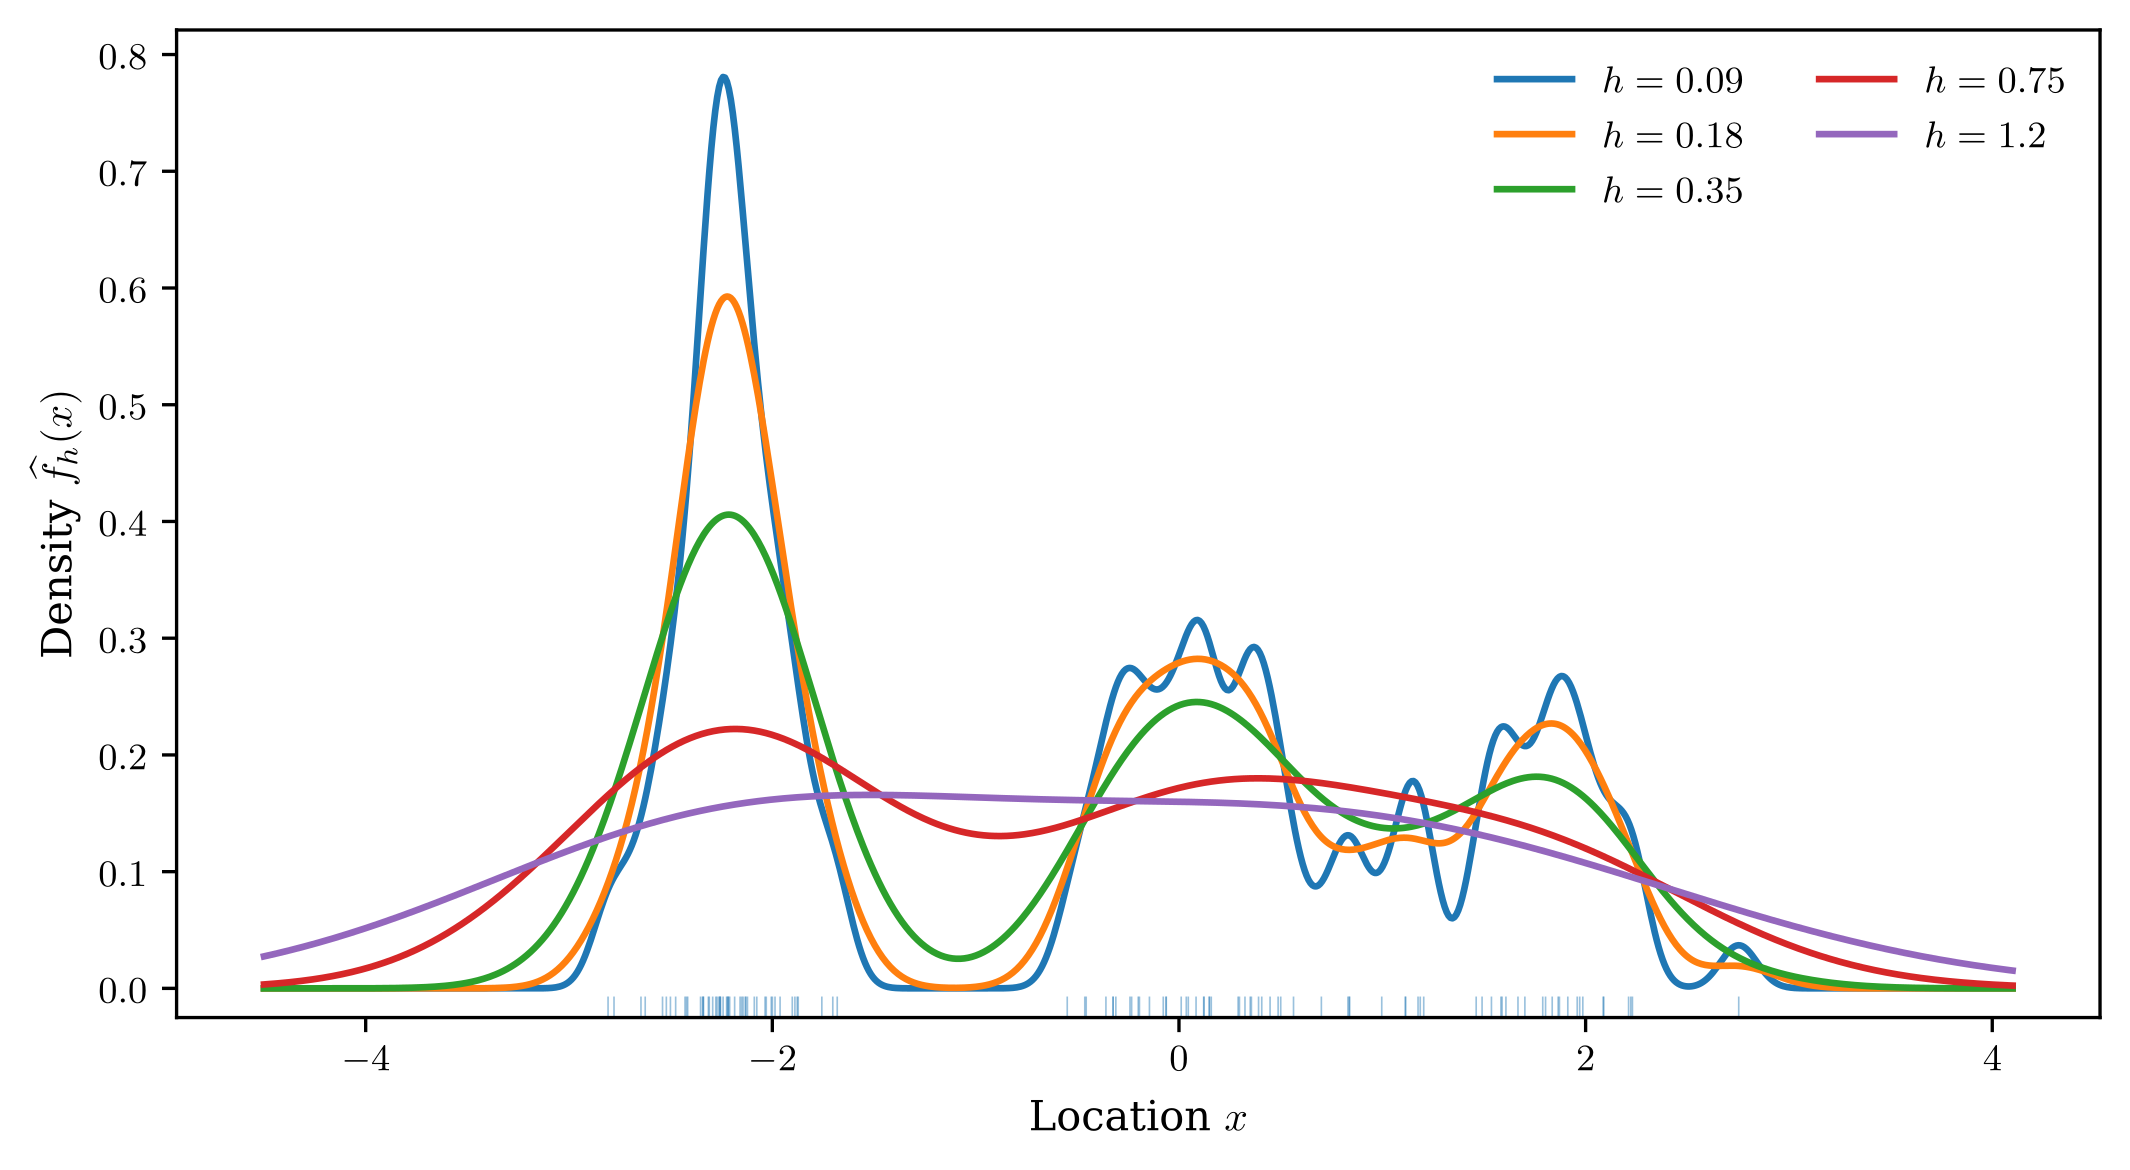
\includegraphics[width=\textwidth]{figures/kde_path.png}
  %\resizebox{\textwidth}{!}{\input{figures/kde_path.pgf}}
  \caption{A density path generated by changing the bandwidth of a Gaussian KDE. Small bandwidths reveal sample-level detail; intermediate bandwidths reveal stable modal structure; large bandwidths produce a coarse summary. The important object is often the whole path, not a single curve.}
  \label{fig:kde-path}
\end{figure*}


\subsection{Bias, variance, and the one-bandwidth tradition}
\label{subsec:bias-variance}

Suppose $X_i\sim f$ independently and $K$ is symmetric with second moment matrix $\mu_2(K)I_d$. Then
\[
  \E\{\fhat_h(x)\}=(K_h*f)(x).
\]
If $f$ is smooth, Taylor expansion gives
\begin{equation*}
  \E\{\fhat_h(x)\}-f(x)
  = \frac{h^2\mu_2(K)}{2}\Delta f(x)+o(h^2).
\end{equation*}
Under standard regularity conditions, the pointwise variance satisfies
\begin{equation*}
  \Var\{\fhat_h(x)\}
  = \frac{1}{nh^d}R(K)f(x)+o\{(nh^d)^{-1}\},
\end{equation*}
for $R(K)=\int K^2(u)\dd u$.
Integrated over $x$, this leads to the usual asymptotic mean integrated squared error (AMISE) approximation
\begin{equation}
  \AMISE(h)
  = \frac{h^4\mu_2(K)^2}{4}R(\Delta f)+\frac{R(K)}{nh^d},
  \label{eq:amise}
\end{equation}
where $R(g)=\int g^2$. The minimizer obeys
\begin{equation}
  h_{\AMISE}\asymp n^{-1/(d+4)}.
  \label{eq:amise-rate}
\end{equation}
This classical calculation is indispensable, explaining the bias-variance tradeoff and the curse of dimensionality. But it also encourages a one-bandwidth mindset: choose $h$ and then inspect $\fhat_h$. The density-evolution perspective keeps the calculation while changing the interpretation. Equation \eqref{eq:amise} is a risk approximation for one frame of a movie. It does not by itself answer which features persist across frames.

\subsection{Gaussian KDE as heat flow}
\label{subsec:kde-heat}

For the Gaussian kernel, KDE is exactly a diffusion. Let
\begin{equation*}
  \varphi_t(x)=(2\pi t)^{-d/2}\exp\left(-\frac{\|x\|^2}{2t}\right),
  \qquad t>0.
\end{equation*}
Define
\begin{equation*}
  \fhat_t(x)=\frac{1}{n}\sum_{i=1}^n \varphi_t(x-X_i),
\end{equation*}
where $t=h^2$. Since
\[
  \partial_t\varphi_t=\frac12\Delta\varphi_t,
\]
linearity gives
\begin{equation*}  \partial_t\fhat_t=\frac12\Delta\fhat_t,
  \qquad
  \fhat_t\to\Emp\quad\text{weakly as }t\downarrow0.
\end{equation*}
Thus a Gaussian KDE is the heat evolution of empirical point masses. 
This identity is the mathematical heart of the density-evolution view:
kernel smoothing is not just a recipe for drawing a smooth curve, but a
Markov semigroup acting on a probability measure.

The same identity also explains why the Gaussian kernel has a special role in scale-space theory. In image analysis, the Gaussian scale-space representation arises from axioms such as linearity, translation invariance, semigroup structure, and non-enhancement of local extrema in one dimension \citep{witkin_1983_ScalespaceFiltering, koenderink_1984_StructureImages, babaud_1986_UniquenessGaussianKernel, lindeberg_1994_ScalespaceTheoryBasic}. In statistics, the same semigroup gives a family of density estimates indexed by resolution.

\subsection{From density values to density features}
\label{subsec:kde-features}

Classical risk measures such as \eqref{eq:amise} quantify error in density values. Many uses of density estimation, however, are feature-driven: how many modes are present, where are the high-density regions, is there a ridge or filament, and which observations lie in low-density regions? A density path makes these questions scale-dependent.

Denote by $M(h)$ the number of modes of $\fhat_h$. For small $h$, $M(h)$ may be close to $n$ or may reflect sample-level noise. For large $h$, $M(h)$ may be one. The practically interesting modes often live at intermediate scales. A bandwidth chosen to minimize integrated squared error need not be the bandwidth that best reveals modal structure. This is why multimodality testing, bump hunting, and scale-space methods evolved alongside classical bandwidth selection.





%----------------------------------------------------------------------------
\section{Scale space, critical bandwidths, mode trees, and SiZer}
\label{sec:scale-space}

Scale space treats smoothing scale as a coordinate. Instead of plotting one curve $x\mapsto\fhat_h(x)$, one studies the surface
\[
  (x,h)\mapsto\fhat_h(x)
\]
or its derivatives. This idea is old in computer vision and signal processing \citep{witkin_1983_ScalespaceFiltering, koenderink_1984_StructureImages, lindeberg_1994_ScalespaceTheoryBasic}, but it has a distinctly statistical form in critical-bandwidth testing, mode trees, and SiZer.

\subsection{Critical bandwidths and multimodality}
\label{subsec:critical-bandwidth}

In one dimension with a Gaussian kernel, increasing $h$ tends to simplify the density. A central object in Silverman's multimodality method is the critical bandwidth
\begin{equation*}
  h_k = \inf\{h>0: \fhat_h \text{ has at most }k\text{ modes}\}.
\end{equation*}
Large $h_k$ is evidence that at least $k+1$ modes are needed to explain the sample. Silverman's test uses the distribution of $h_k$ under a null model with $k$ modes, and later work refined calibration and related excess-mass approaches \citep{silverman_1981_UsingKernelDensity, polonik_1995_MeasuringMassConcentrations, hall_2001_CalibrationSilvermansTest, fisher_2001_ModeTestingExcess, ameijeiras-alonso_2019_ModeTestingCritical}.

From the evolution viewpoint, $h_k$ is not merely a test statistic, but a scale at which the topology of the modal landscape changes. If $h$ increases, small modes disappear or merge. If $h$ decreases, branches split. This is the first example of a feature lifetime: a mode is not simply present or absent; it is present over a scale interval.

\subsection{Mode trees}
\label{subsec:mode-trees}

The mode tree plots mode locations as a function of bandwidth \citep{minnotte_1993_ModeTreeTool}. Define
\[
  \calM(h)=\{x:\fhat_h'(x)=0,\ \fhat_h''(x)<0\}
\]
in one dimension. The mode tree displays the set
\begin{equation*}
  \mathcal T_{\mathrm{mode}}=\{(x,h):x\in\calM(h)\}.
\end{equation*}
Branches that persist across a wide range of bandwidths are more interpretable than short branches that appear only at fine scales. The logic is similar to persistent homology, but the features are critical points of a smoothed density rather than homology classes of a filtration.

\begin{figure}[t]
  \centering
  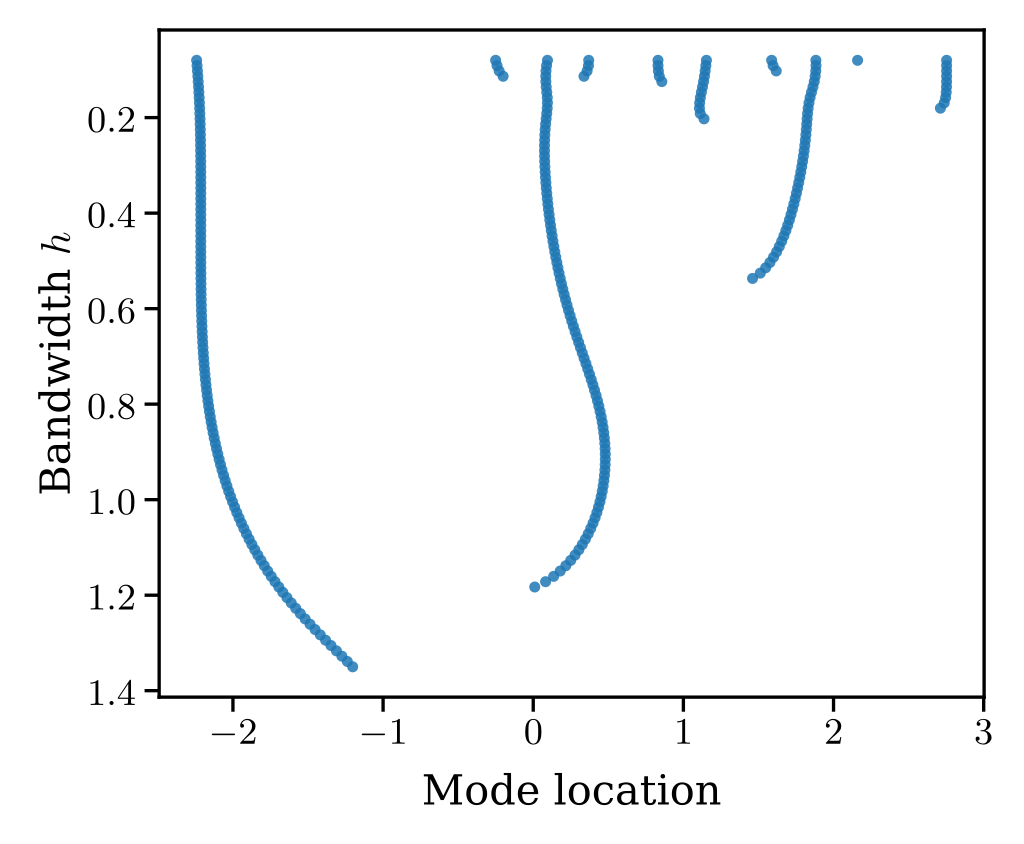
\includegraphics[width=.55\textwidth]{figures/mode_tree.png}
  %\resizebox{.55\columnwidth}{!}{\input{figures/mode_tree.pgf}}
  \caption{A mode-tree summary of the same one-dimensional sample as in Figure~\ref{fig:kde-path}. Each point marks a mode location for a bandwidth. The vertical axis is inverted so that fine scales appear near the top. Persistent branches correspond to modes that survive substantial smoothing.}
  \label{fig:mode-tree}
\end{figure}

Mode trees encourage a different interpretation of multimodality. The question ``how many modes?'' becomes ``which modal branches persist, and how should persistence be calibrated against sampling noise?'' Minnotte's later work on mode existence and related tests further developed this inferential direction \citep{minnotte_1997_NonparametricTestingExistence}. In multivariate settings, the geometry is richer: modes can move through space, saddles and ridges matter, and the number of modes of a Gaussian mixture need not behave monotonically under smoothing \citep{carreira-perpinan_2003_NumberModesGaussian, ray_2005_TopographyMultivariateNormal}.

The following theorem formalizes the local branch structure behind a mode tree. It is a direct application of the implicit function theorem, but the statement is useful because it identifies the only local mechanisms by which a mode branch can fail to continue: a degenerate Hessian or a boundary/infinity event.

\begin{theorem}[Local motion of modes]
\label{thm:mode-motion}
Let $U\subset\R^d$ be open and let $I\subset\R$ be an interval.
Suppose $f:U\times I\to\R$ is twice continuously differentiable in $x$,
differentiable in $t$, and that
\[
  F(x,t)=\nabla_x f(x,t)
\]
is continuously differentiable in $(x,t)$. Assume also that mixed
derivatives commute, so that
\[
  \partial_t\nabla_x f=\nabla_x\partial_t f.
\]
Let $(x_0,t_0)\in U\times I$ satisfy
\[
  \nabla_x f(x_0,t_0)=0,
  \qquad
  H_0:=\nabla_x^2 f(x_0,t_0) \text{ is nonsingular}.
\]
Then there are neighborhoods $V$ of $x_0$ and $J$ of $t_0$, and a unique
continuously differentiable curve $m:J\to V$, such that
\[
  m(t_0)=x_0,
  \qquad
  \nabla_x f(m(t),t)=0
  \quad(t\in J).
\]
Moreover,
\[
  \dot m(t)
  =-\{\nabla_x^2 f(m(t),t)\}^{-1}
     \nabla_x\{\partial_t f(m(t),t)\}.
\]
If $H_0$ is negative definite, then after possibly shrinking $J$, the
curve consists of local modes. For heat flow,
\(\partial_t f_t=(1/2)\Delta f_t\), this becomes
\[
  \dot m(t)
  =-\frac12\{\nabla_x^2 f_t(m(t))\}^{-1}
    \nabla_x\Delta f_t(m(t)).
\]
Consequently, fix \(t_0\in I\) and a compact set \(K\subset U\). If no
critical point of \(f(\cdot,t_0)\) lies on \(\partial K\), and all
critical points of \(f(\cdot,t_0)\) in \(K\) are nondegenerate, then for
all \(t\) sufficiently close to \(t_0\), the number and Morse type of
critical points in \(K\) are unchanged.
\end{theorem}

\subsection{SiZer and significant features across scale}
\label{subsec:sizer}

SiZer was introduced to display statistically significant features in smooth curve estimates across location and scale \citep{chaudhuri_1999_SiZerExplorationStructures, chaudhuri_2000_ScaleSpaceView}. For density estimation, the first derivative is central. If $\fhat_h'(x)>0$, the density is locally increasing while $\fhat_h'(x)<0$ indicates decrease. A mode occurs near a transition from positive to negative derivative.

A simplified version of the inferential calculation is as follows. Let
\[
  \fhat_h'(x)=\frac{1}{nh^2}\sum_{i=1}^n K'\left(\frac{x-X_i}{h}\right)
\]
in one dimension. Under regularity conditions, a standardized statistic
\[
  Z_h(x)=\frac{\fhat_h'(x)-\E\{\fhat_h'(x)\}}{\widehat{\operatorname{se}}\{\fhat_h'(x)\}}
\]
is approximately Gaussian. SiZer uses simultaneous inference ideas to color regions of the $(x,h)$ plane where the derivative is significantly positive, significantly negative, or not significantly different from zero. The resulting display communicates which features are statistically supported at which scales, rather than forcing a single smoothing choice.

This is perhaps the most direct precursor of density-evolution inference. It recognizes that the target of inference is not only $f(x)$, but the qualitative structure of an evolving estimate.

\subsection{Causality and the multivariate caveat}
\label{subsec:causality}

A guiding principle in scale-space theory is causality: moving to coarser
scales should not create new meaningful structure. In one dimension, Gaussian smoothing has a variation-diminishing property related to total positivity, and the number of modes cannot increase under Gaussian convolution under suitable conditions \citep{schoenberg_1951_PolyaFrequencyFunctions, silverman_1981_UsingKernelDensity}. This justifies the interpretation that increasing bandwidth merges or removes modes.

In dimensions $d\ge2$, the picture is more delicate. Gaussian blurring can create modes for general functions, and the number of modes of a Gaussian mixture can behave in surprising ways \citep{carreira-perpinan_2003_NumberModesGaussian}. This does not invalidate multiscale density analysis, but it weakens the simple one-dimensional story. A major open question is whether useful classes of multivariate density evolutions can be constructed with a strong causality property for modes, ridges, or topological summaries.


%----------------------------------------------------------------------------
\section{Mean shift, modes, and gradient flows of the KDE}
\label{sec:mean-shift}

The modal structure of a KDE is linked to gradient ascent. This connection is important both computationally and conceptually, because it turns modes into attractors of a vector field.

Consider a radial kernel
\[
  K(u)=c_k k(\|u\|^2)
\]
with profile $k$, and define $g(r)=-k'(r)$. The KDE is
\[
  \fhat_h(x)=\frac{c_k}{nh^d}\sum_{i=1}^n k\left(\frac{\|x-X_i\|^2}{h^2}\right).
\]
Differentiating gives
\begin{align*}
  \nabla \fhat_h(x)
  &= \frac{2c_k}{nh^{d+2}}
     \sum_{i=1}^n (X_i-x)\,g\left(\frac{\|x-X_i\|^2}{h^2}\right)\\
  &= C_h(x)\left\{m_h(x)-x\right\},
\end{align*}
where
\begin{equation*}
  m_h(x)=\frac{\sum_{i=1}^n X_i g(\|x-X_i\|^2/h^2)}{\sum_{i=1}^n g(\|x-X_i\|^2/h^2)}
\end{equation*}
and $C_h(x)$ is a positive scalar factor when the denominator is nonzero. Thus the mean-shift vector
\begin{equation*}
  m_h(x)-x
\end{equation*}
is proportional to the gradient of the KDE. For the Gaussian kernel, it is also proportional to the gradient of the log density:
\begin{equation}
  m_h(x)-x = h^2\nabla\log\fhat_h(x).
  \label{eq:gaussian-mean-shift-score}
\end{equation}
This identity links three ideas: KDE modes, score fields, and iterative clustering. The fixed points of $m_h$ are critical points of the density; stable fixed points correspond to modes under suitable conditions. Mean-shift clustering assigns points to basins of attraction of modes 
\citep{fukunaga_1975_EstimationGradientDensity, cheng_1995_MeanShiftMode, comaniciu_2002_MeanShiftRobust, azzalini_2007_ClusteringNonparametricDensity}.

For density evolution, mean shift shows that each scale $h$ has its own gradient flow. As $h$ varies, both the vector field and its attractor basins evolve. This suggests a dynamic view of density-based clustering that clusters are not fixed partitions, but basins of attraction that appear, merge, and disappear across scale.


%----------------------------------------------------------------------------
\section{From kernels to mixtures}
\label{sec:mixtures}

Kernel estimates and Gaussian mixtures are often taught separately: the former as nonparametric smoothing, the latter as parametric or semiparametric modeling. Yet the Gaussian KDE is a special Gaussian mixture,
\begin{equation*}
  \fhat_h(x)=\sum_{i=1}^n \frac1n\,\Normal(x\mid X_i,h^2I_d).
\end{equation*}
A general Gaussian mixture is
\begin{equation*}
  f_K(x)=\sum_{k=1}^K \pi_k\,\Normal(x\mid \mu_k,\Sigma_k),
  \quad
  \pi_k\ge0,~ \sum_{k=1}^K\pi_k=1.
\end{equation*}
The KDE corresponds to $K=n$, equal weights, fixed means, and common covariance. A single Gaussian corresponds to $K=1$. This yields a second density-evolution axis: mixture complexity.

\subsection{Discrete complexity paths}
\label{subsec:mixture-paths}

Finite mixtures give a discrete path
\[
  K=1,2,3,\ldots,
\]
where $K$ is the number of components. Model selection criteria, penalized likelihood, minimum message length, reversible-jump Markov chain Monte Carlo, and Bayesian nonparametric mixtures all provide ways to move along or average over this path \citep{lindsay_1995_MixtureModelsTheory, richardson_1997_BayesianAnalysisMixtures, figueiredo_2002_UnsupervisedLearningFinite, fraley_2002_ModelBasedClusteringDiscriminant, mclachlan_2019_FiniteMixtureModels}. This path is different from the KDE bandwidth path. Bandwidth controls smoothing continuously; $K$ controls representational complexity discretely. Both are attempts to move between local detail and global summary.

The phrase ``component'' must be used carefully. A mixture component need not correspond to a mode, and a mixture with $K$ Gaussian components can have more or fewer than $K$ modes depending on dimension and covariance structure \citep{carreira-perpinan_2003_NumberModesGaussian, ray_2005_TopographyMultivariateNormal}. From the density-evolution perspective, mixture components are a representation of the path, while modes are features of the resulting density landscape.

\subsection{Kernel-to-mixture reduction}\label{subsec:kernel-to-mixture}

A particularly close precursor is the kernel-to-mixture reduction work of Scott and Szewczyk \citep{scott_2001_KernelsMixtures}. It treats kernel estimators as large mixtures and studies how to collapse components recursively to obtain a more parsimonious mixture representation. At a high level, one starts with a KDE-like mixture and repeatedly merges components that are close according to a density-similarity measure. If two Gaussian components with weights $\pi_a,\pi_b$, means $\mu_a,\mu_b$, and covariances $\Sigma_a,\Sigma_b$ are merged, a moment-matched replacement has weight
\[
  \pi=\pi_a+\pi_b,
\]
mean
\[
  \mu=\frac{\pi_a\mu_a+\pi_b\mu_b}{\pi},
\]
and covariance
\begin{align*}
  \Sigma
  &=\frac{\pi_a}{\pi}\left\{\Sigma_a+(\mu_a-\mu)(\mu_a-\mu)^T\right\}\\
  &+\frac{\pi_b}{\pi}\left\{\Sigma_b+(\mu_b-\mu)(\mu_b-\mu)^T\right\}.  
\end{align*}
This operation preserves the first two moments of the pair and creates a path from many components to fewer components. Related ideas appear in alternating kernel and mixture estimates \citep{priebe_2000_AlternatingKernelMixture} and in broader mixture-reduction algorithms.

It is worth emphasizing that this path differs from heat flow. Heat flow increases component variance while keeping component centers fixed. Mixture reduction changes the representation by merging centers and covariances. Both can be viewed as density evolutions, but they encode different notions of simplification.

\subsection{Mixing distributions}
\label{subsec:mixing-distributions}

A general mixture can be written as
\begin{equation*}
  f_G(x)=\int \Normal(x\mid \theta)\,\dd G(\theta),
\end{equation*}
where $G$ is a mixing distribution over parameters $\theta=(\mu,\Sigma)$ or a subset thereof. Then a single Gaussian is obtained when $G$ is a point mass, a finite mixture when $G$ is discrete with $K$ atoms, and a KDE when $G$ is the empirical distribution over locations with fixed covariance. This representation connects KDEs, finite mixtures, nonparametric maximum likelihood for mixtures, and Bayesian nonparametric mixtures  \citep{kiefer_1956_ConsistencyMaximumLikelihood, ferguson_1973_BayesianAnalysisNonparametric, lo_1984_ClassBayesianNonparametric, escobar_1995_BayesianDensityEstimation, lindsay_1995_MixtureModelsTheory}.

The density-evolution viewpoint treats $G$ itself as an object that may evolve. Atoms may split or merge, weights may shrink, covariance may inflate, and the mixing distribution may move from empirical discreteness toward a low-complexity summary.

%----------------------------------------------------------------------------
\section{Diffusion, semigroups, and Gaussianization}
\label{sec:diffusion}

The heat interpretation of Gaussian KDE suggests a broader class of density evolutions based on Markov processes. Let $(X_t)_{t\ge0}$ be a diffusion with generator
\begin{equation*}
\calL\phi(x)=b(x)\cdot\nabla\phi(x)+\frac12\tr\{a(x)\nabla^2\phi(x)\},
\end{equation*}
where $a(x)=\sigma(x)\sigma(x)^T$. If $f_t$ is the density of $X_t$, it satisfies the Fokker--Planck equation
\begin{equation}
  \partial_t f_t
  = -\nabla\cdot\{b f_t\}+\frac12\sum_{i,j}\partial_{ij}\{a_{ij}f_t\}
  = \calL^* f_t.
  \label{eq:fokker-planck}
\end{equation}
Thus a density evolution may be generated by a semigroup $P_t^*$:
\[
  f_t=P_t^* f_0.
\]
For empirical $f_0=\Emp$, this is understood weakly; for $t>0$ the distribution may have a smooth density.

\subsection{Adaptive diffusion}
\label{subsec:adaptive-diffusion}

Classical KDE uses the same smoothing everywhere. Adaptive density estimation modifies the amount of smoothing according to local data density \citep{abramson_1982_BandwidthVariationKernel, terrell_1992_VariableKernelDensity}. Diffusion-based KDE provides a principled partial differential equation (PDE) route. One chooses a diffusion process whose local behavior adapts to a pilot estimate, support constraints, or boundary behavior. Diffusion formulations show how adaptive KDE can be constructed from linear diffusion processes, yielding bandwidth selectors and boundary-aware estimators \citep{botev_2010_KernelDensityEstimation}.


For density evolution, adaptive diffusion raises a fundamental question: should scale be global or local? A single bandwidth $h$ imposes one resolution on all regions. A spatially varying diffusion tensor can smooth aggressively in low-information regions and gently near sharp features. The cost is that the evolution operator becomes model-dependent and less transparent.

\subsection{A path from empirical measure to fitted Gaussian}
\label{subsec:ou-path}

Heat flow has an inconvenient endpoint for the original motivation of moving from many local components to one Gaussian: as $t\to\infty$, heat flow spreads mass over all of $\R^d$ rather than converging to the sample Gaussian. An Ornstein--Uhlenbeck-type construction gives a more direct path.

Let
\[
  \bar X=\frac1n\sum_{i=1}^n X_i,
  \qquad
  S=\frac1n\sum_{i=1}^n (X_i-\bar X)(X_i-\bar X)^T.
\]
Assume first that $S$ is positive definite. Let $a_t=e^{-t}$ and define
\begin{equation}
  g_t(x)=\frac1n\sum_{i=1}^n
  \Normal\left(x\mid \bar X+a_t(X_i-\bar X),\ (1-a_t^2)S\right).
  \label{eq:ou-gaussianization}
\end{equation}
At $t=0$, the covariance term vanishes and $g_t$ converges weakly to $\Emp$. For $t>0$, $g_t$ is an $n$-component Gaussian mixture. As $t\to\infty$, all component means collapse to $\bar X$ and the covariance becomes $S$, so
\begin{equation*}
  g_t \to \Normal(\bar X,S).
\end{equation*}
Moreover, the mean and covariance are preserved for all $t$:
\[
  \E_{g_t}(X)=\bar X,
  \qquad
  \Cov_{g_t}(X)=a_t^2S+(1-a_t^2)S=S.
\]
This path can be generated by an OU process after whitening by $S^{-1/2}$. In standardized coordinates, $Y_t=e^{-t}Y_0+\sqrt{1-e^{-2t}}Z$ with $Z\sim\Normal(0,I_d)$. Transforming back gives \eqref{eq:ou-gaussianization}.

The next result explains why this formulation is more than an arbitrary interpolation. In a natural class of linear Gaussian evolutions that use the current mean and covariance of the distribution, the OU form is forced by moment preservation and the semigroup property, up to a constant rescaling of time. The assumption of positive definite covariance can be relaxed by working on the affine span of the distribution or by using a regularized covariance. We state the clean full-rank version. 

The finite-third-moment assumption is used only to identify the coefficient
of the non-Gaussian part through third central moments.
\begin{theorem}[Characterization of the moment-preserving Gaussianization semigroup]
\label{thm:ou-characterization}
Let $\mathcal P_3^+$ be the class of probability measures on $\R^d$ with finite third moments and positive definite covariance. For $P\in\mathcal P_3^+$, write $m_P$ and $S_P$ for its mean and covariance. Suppose a family of maps $(T_t)_{t\ge0}$ has the form
\begin{equation}
  T_tP
  =\mathcal{L}\{m_P+a(t)(X-m_P)+b(t)Z_P\},
  \label{eq:linear-gaussian-class-main}
\end{equation}
where $X\sim P$, $Z_P\sim\Normal(0,S_P)$ is independent of $X$, $a,b$ are continuous functions, $a(0)=1$, $b(0)=0$, $b(t)\ge0$, and $0\le a(t)\le1$. Assume that:
\begin{enumerate}
\item $T_t$ preserves mean and covariance for every $P\in\mathcal P_3^+$;
\item $(T_t)_{t\ge0}$ is a semigroup on $\mathcal P_3^+$, that is, $T_{s+t}P=T_s(T_tP)$ for all $s,t\ge0$ and all $P\in\mathcal P_3^+$;
\item the family is not the identity, meaning $a(t)<1$ for at least one $t>0$.
\end{enumerate}
Then there is a constant $c>0$ such that
\begin{equation*}
  a(t)=e^{-ct},
  \qquad
  b(t)=\sqrt{1-e^{-2ct}}.
\end{equation*}
Thus, after the time change $t\mapsto ct$, \eqref{eq:linear-gaussian-class-main} is exactly the OU Gaussianization path
\[
  T_tP
  =\mathcal{L}\{m_P+e^{-t}(X-m_P)+\sqrt{1-e^{-2t}}Z_P\}.
\]
\end{theorem}

A second structural fact is that shared-covariance Gaussian mixtures have a simple log-concavity certificate. This gives explicit terminal times after which heat-flow and OU density evolutions can no longer have multiple modes or nonconvex superlevel sets. The theorem is deliberately stated for general unequal weights because the proof uses only the common-covariance mixture geometry.

\begin{theorem}[Terminal log-concavity for shared-covariance mixtures]
\label{thm:terminal-logconcavity}
Let
\begin{equation*}
  f(x)=\sum_{i=1}^n \pi_i\,\varphi_\Sigma(x-\mu_i),
  \quad
  \pi_i>0, ~\sum_{i=1}^n\pi_i=1,~
  \Sigma\succ0.
\end{equation*}
Define posterior weights
\[
  w_i(x)=\frac{\pi_i\varphi_\Sigma(x-\mu_i)}{f(x)},
  \qquad
  \bar\mu_w(x)=\sum_i w_i(x)\mu_i,
\]
and the weighted covariance matrix of component means
\[
  C_w(x)=\sum_i w_i(x)\{\mu_i-\bar\mu_w(x)\}\{\mu_i-\bar\mu_w(x)\}^T.
\]
Then
\begin{equation*}
  \nabla^2\log f(x)
  =-\Sigma^{-1}+\Sigma^{-1}C_w(x)\Sigma^{-1}.
\end{equation*}
Consequently, $f$ is log-concave if $C_w(x)\preceq\Sigma$ for all $x$, and strictly log-concave if $C_w(x)\prec\Sigma$ for all $x$. In particular, if there is a point $c\in\R^d$ such that
\begin{equation*}
  \max_i \|\Sigma^{-1/2}(\mu_i-c)\|^2<1,
\end{equation*}
then $f$ is strictly log-concave.

The following consequences hold.
\begin{enumerate}
\item For the heat-flow KDE
\[
  \widehat f_t(x)=\frac1n\sum_{i=1}^n\varphi_{tI_d}(x-X_i),
\]
if $\max_i\|X_i-c\|^2\le R^2$, then $\widehat f_t$ is strictly log-concave for every $t>R^2$.
\item For the OU path \eqref{eq:ou-gaussianization}, assume $S\succ0$ and define
\[
  R_S^2=\max_i (X_i-\bar X)^T S^{-1}(X_i-\bar X).
\]
Then $g_t$ is strictly log-concave whenever
\begin{equation*}
  t>\frac12\log(1+R_S^2).
\end{equation*}
\end{enumerate}
At those times the density has a unique mode, and all positive-level
superlevel sets are convex.
\end{theorem}

\begin{figure*}[t]
  \centering
  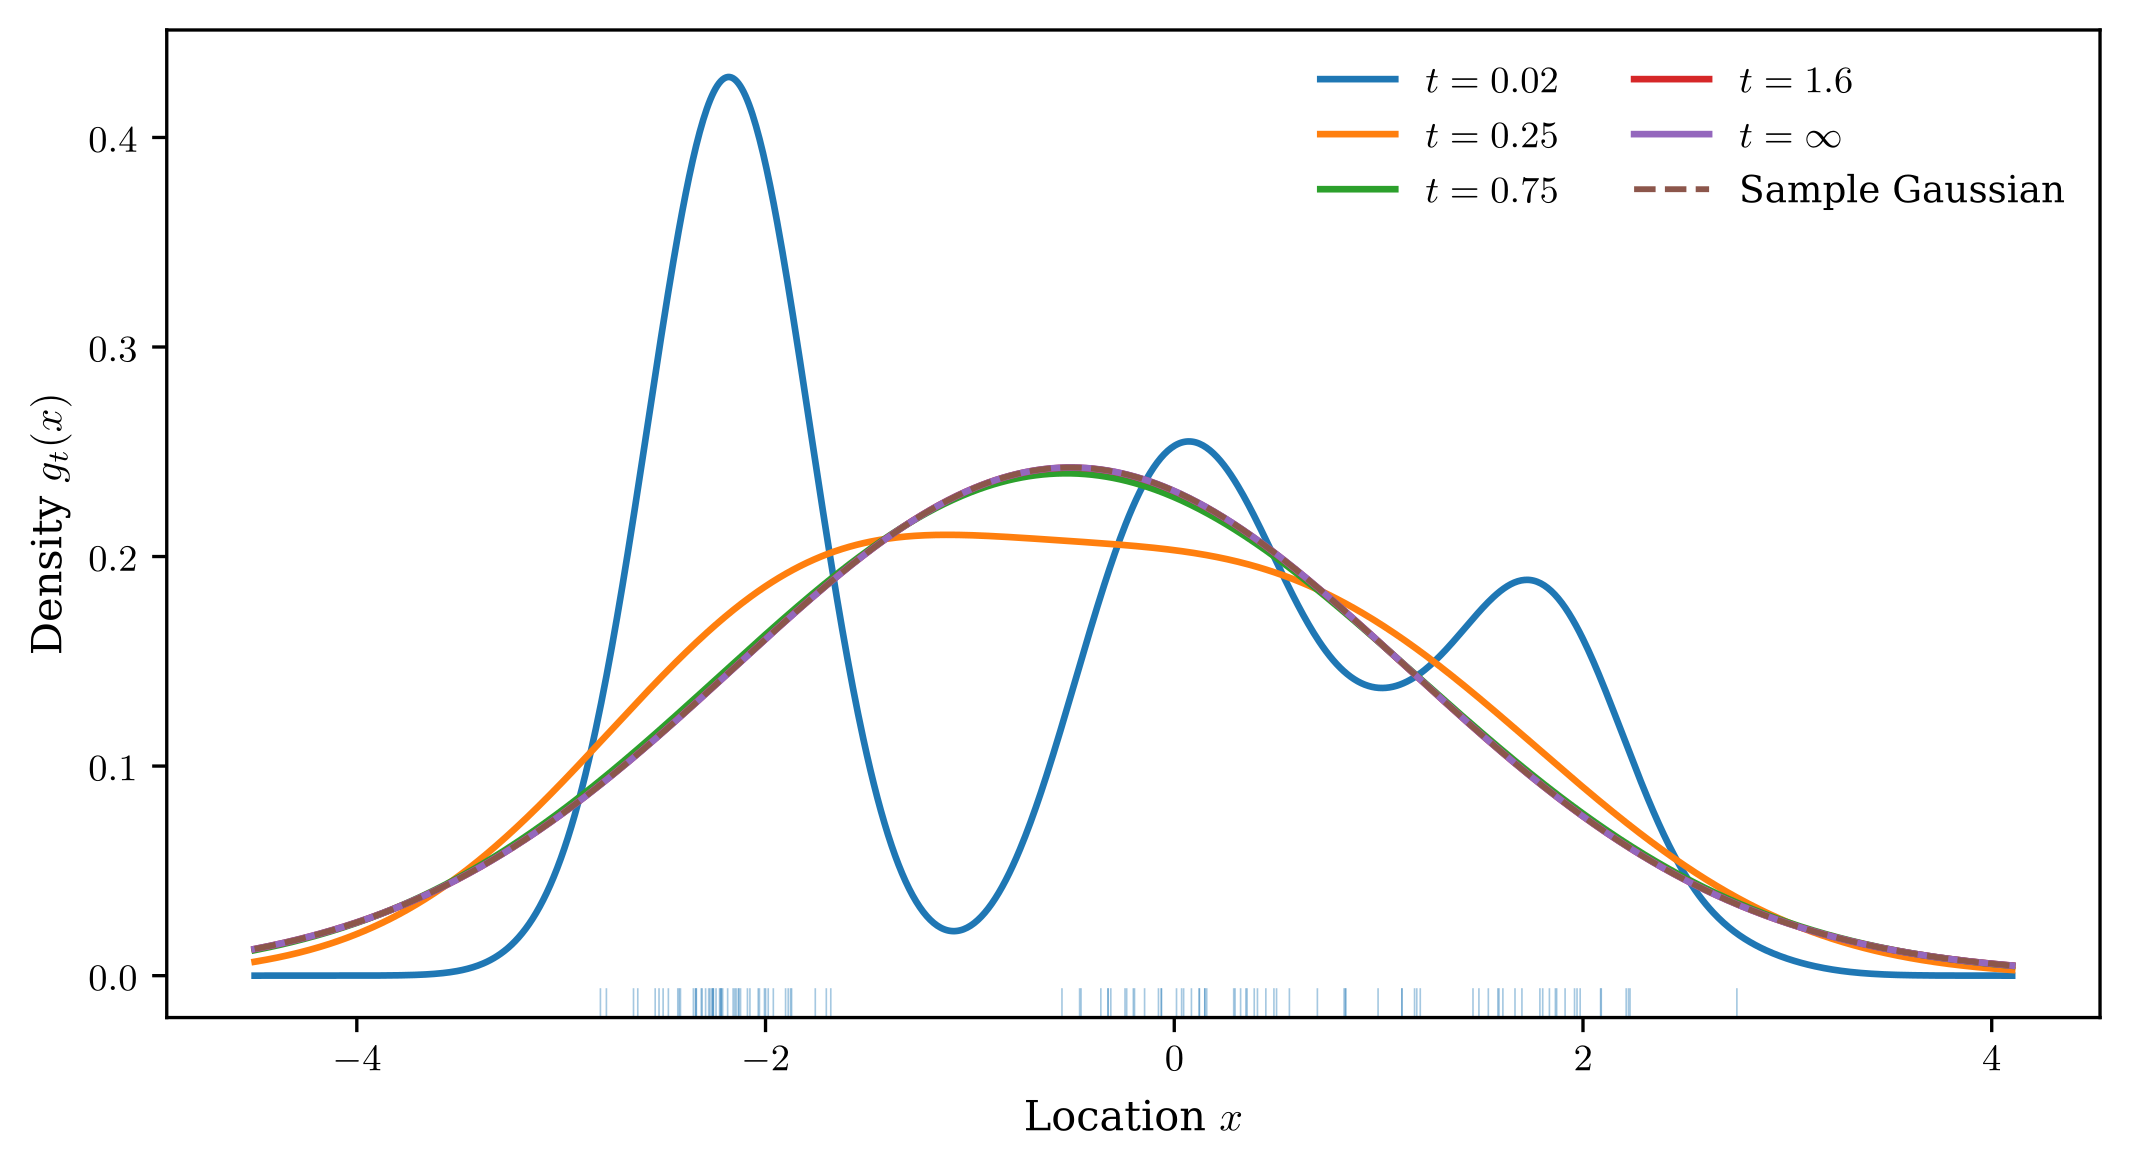
\includegraphics[width=\textwidth]{figures/ou_path.png}
  %\resizebox{\textwidth}{!}{\input{figures/ou_path.pgf}}
  \caption{An Ornstein--Uhlenbeck-type Gaussianization path. Unlike ordinary heat flow, this path preserves the sample mean and covariance and converges to the fitted Gaussian. It provides a mathematically explicit continuum from empirical spikes to an $n$-component mixture to a single Gaussian summary.}
  \label{fig:ou-path}
\end{figure*}

This construction is useful as a conceptual example even if it is not always the desired estimator. It is affine-equivariant, has interpretable endpoints, and preserves the first two moments. In high dimensions with singular $S$, one can use a regularized covariance $S_\epsilon=S+\epsilon I_d$ or work in the empirical principal subspace. The open statistical question is whether such Gaussianization paths can be used for model selection, feature persistence, or hypothesis testing in a way that complements KDE scale space.

\subsection{Entropy and information dissipation}
\label{subsec:entropy}

Diffusion paths often have monotone information quantities. For heat flow, let $f_t=f_0*\varphi_t$ and define differential entropy
\[
  H(f_t)=-\int f_t\log f_t\dd x
\]
and Fisher information
\[
  I(f_t)=\int \|\nabla\log f_t\|^2 f_t\dd x.
\]
A formal integration-by-parts calculation gives de Bruijn's identity
\begin{equation*}
  \frac{\dd}{\dd t}H(f_t)=\frac12 I(f_t).
\end{equation*}
Indeed,
\begin{align*}
  \frac{\dd}{\dd t}H(f_t)
  &= -\int (\partial_t f_t)\log f_t\dd x \\
  &= -\frac12\int (\Delta f_t)\log f_t\dd x \\
  &= \frac12\int \frac{\|\nabla f_t\|^2}{f_t}\dd x
   = \frac12 I(f_t),
\end{align*}
assuming boundary terms vanish. Thus heat flow increases entropy and smooths information. The OU semigroup has an analogous relative-entropy dissipation identity with respect to its Gaussian invariant distribution  \citep{bakry_2014_AnalysisGeometryMarkov}. The Wasserstein gradient-flow formulation of Fokker--Planck equations provides another geometric interpretation of such evolutions \citep{jordan_1998_VariationalFormulationFokkerPlanck, villani_2009_OptimalTransportOld}.

For statistics, these identities suggest continuous measures of distributional complexity. Instead of counting modes or components, one can summarize the path through integrated Fisher information, entropy production, or changes in relative entropy. These summaries may be less visually immediate than mode trees, but they can be stable in high dimension and connect density estimation to information theory \citep{stam_1959_InequalitiesSatisfiedQuantities, cover_2005_ElementsInformationTheory}.




%----------------------------------------------------------------------------
\section{Level sets, cluster trees, and topology}
\label{sec:levelsets}

Modes summarize local maxima. Many clustering and topological questions are better expressed through level sets. For a density $f$ and a level $\lambda$, define the upper level set
\begin{equation*}
  L_\lambda(f)=\{x\in\R^d:f(x)\ge\lambda\}.
\end{equation*}
As $\lambda$ decreases, components of $L_\lambda(f)$ appear and merge. The collection of these components forms the cluster tree.

\subsection{Cluster trees}
\label{subsec:cluster-trees}

Hartigan's classical density-clustering view defines clusters as high-density connected components \citep{hartigan_1975_ClusteringAlgorithms}. More formally, the cluster tree is
\begin{equation*}
  \mathcal C_f = \{\text{connected components of }L_\lambda(f):\lambda\ge0\},
\end{equation*}
with parent-child relationships induced by set inclusion as $\lambda$ changes. This object records a hierarchy without choosing a fixed number of clusters.

The cluster-tree literature has studied estimation, pruning, and consistency 
\citep{stuetzle_2003_EstimatingClusterTree, stuetzle_2010_GeneralizedSingleLinkage, chaudhuri_2010_RatesConvergenceCluster, chaudhuri_2014_ConsistentProceduresCluster, eldridge_2015_HartiganConsistencyMerge}. Level-set estimation and excess-mass methods provide complementary inferential foundations 
\citep{polonik_1995_MeasuringMassConcentrations, tsybakov_1997_NonparametricEstimationDensity, rigollet_2009_OptimalRatesPlugin, samworth_2010_AsymptoticsOptimalBandwidth, rinaldo_2010_GeneralizedDensityClustering, steinwart_2015_FullyAdaptiveDensitybased}.  Density-based algorithms such as HDBSCAN, a hierarchical density-based clustering method, can also be interpreted as practical cluster-tree approximations  \citep{campello_2015_HierarchicalDensityEstimates}.

Density evolution adds a second axis. Instead of a single estimated density $\fhat$ and level $\lambda$, consider
\begin{equation}
  L_{t,\lambda}=\{x:\fhat_t(x)\ge\lambda\}.
  \label{eq:two-parameter-level-set}
\end{equation}
Now the cluster structure varies with both smoothing scale $t$ and density level $\lambda$. Figure~\ref{fig:levelset-heatmap} illustrates this two-parameter view in one dimension by counting superlevel-set components.

\begin{figure*}[t]
  \centering
  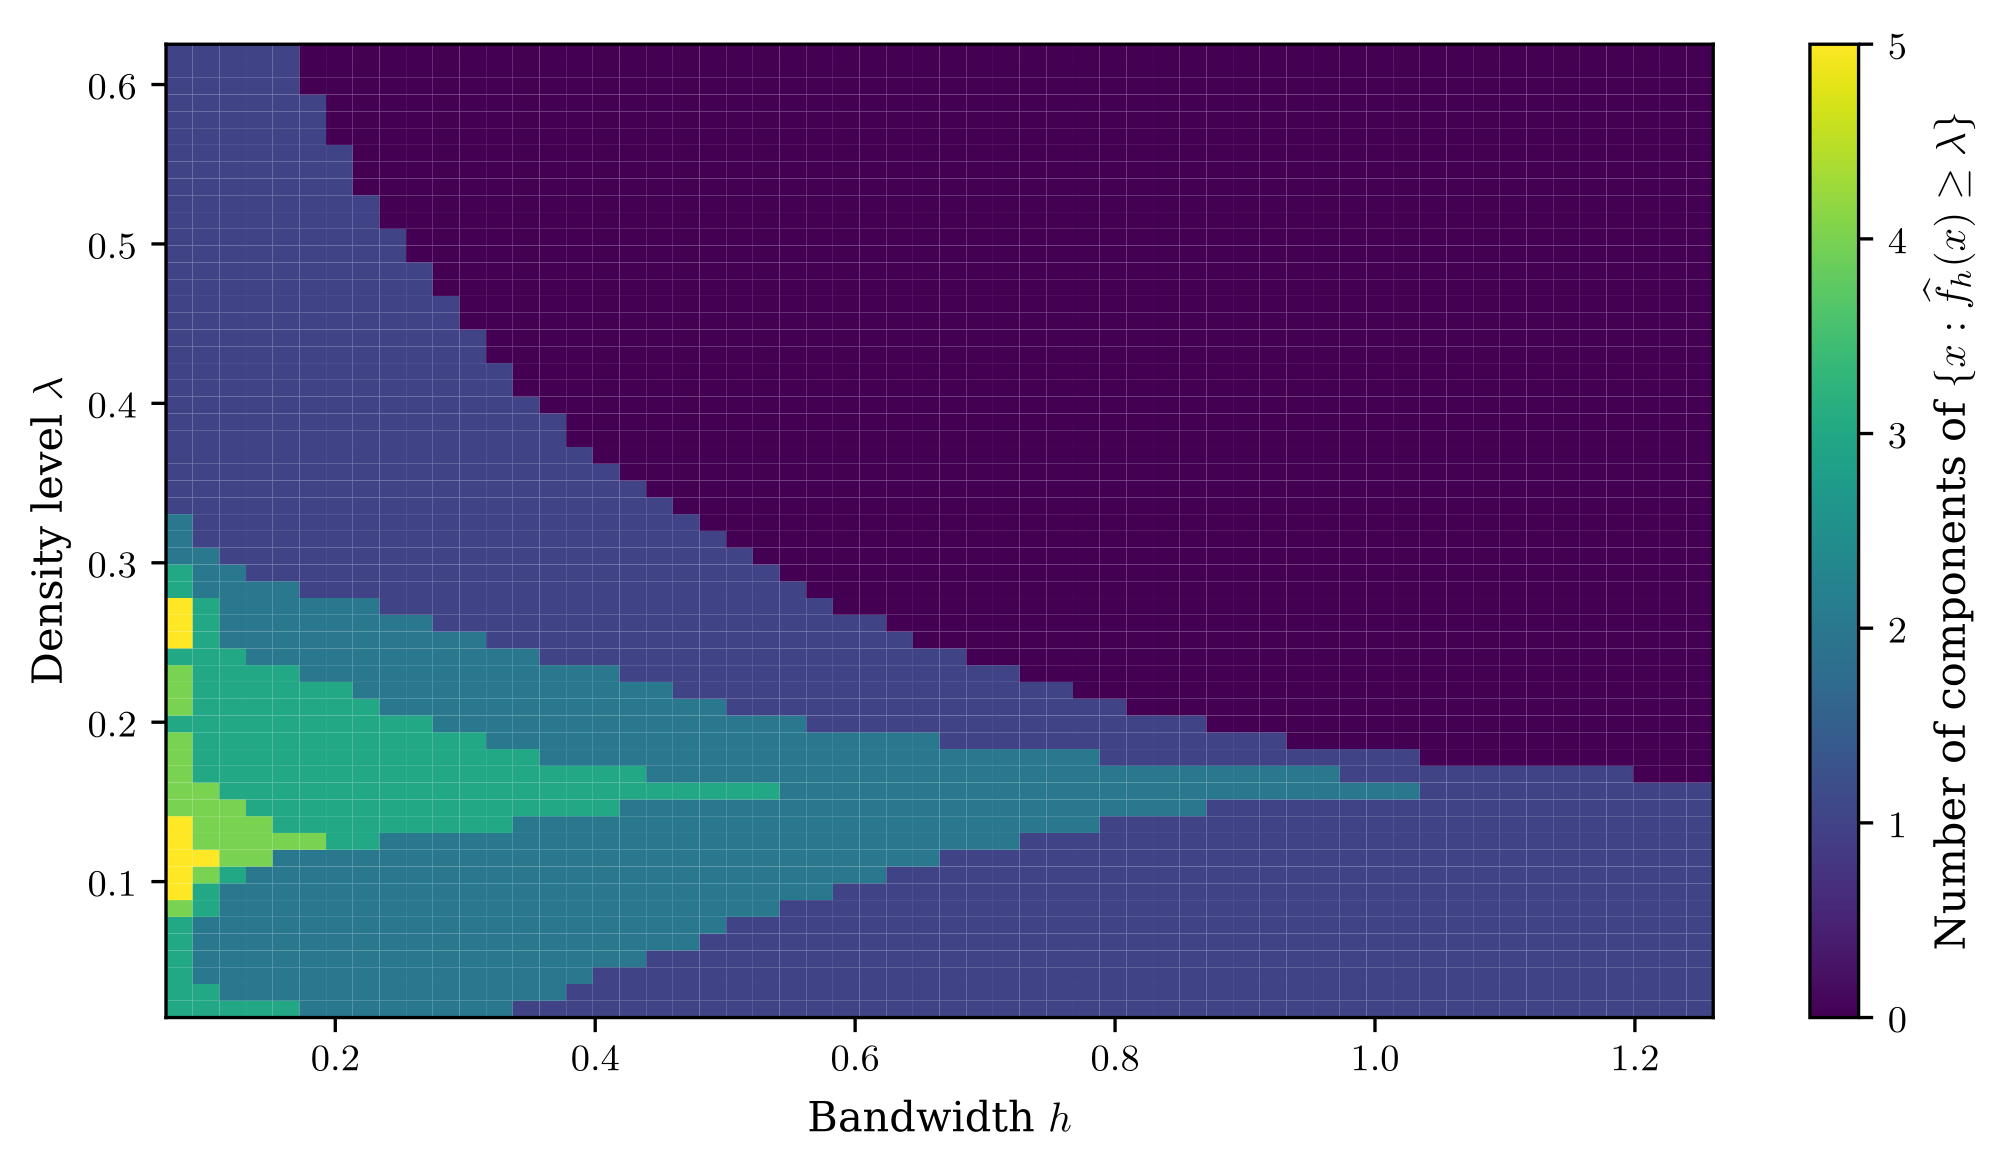
\includegraphics[width=\textwidth]{figures/levelset_heatmap.png}
  %\resizebox{\textwidth}{!}{\input{figures/levelset_heatmap.pgf}}
  \caption{A two-parameter density-evolution summary. Each point records the number of connected components of the superlevel set $\{x:\fhat_h(x)\ge\lambda\}$ for a smoothing bandwidth $h$ and density level $\lambda$. Classical cluster trees vary $\lambda$ for one density. Density evolution also varies the smoothing scale.}
  \label{fig:levelset-heatmap}
\end{figure*}

\subsection{Persistent homology}
\label{subsec:persistence}

Persistent homology studies topological features that are born and die along a filtration \citep{edelsbrunner_2002_TopologicalPersistenceSimplification, carlsson_2009_TopologyData, edelsbrunner_2010_ComputationalTopologyIntroduction, wasserman_2018_TopologicalDataAnalysis}. For density analysis, a natural filtration is given by superlevel sets $L_\lambda(f)$ as $\lambda$ decreases. Zero-dimensional homology tracks connected components and higher-dimensional homology tracks loops, voids, and more complicated structures.

The persistence diagram records birth and death values of topological features. Short-lived features are often interpreted as noise, while long-lived features are treated as signal. This language is closely aligned with mode-tree thinking. The difference is that persistent homology is not restricted to modes and can capture holes and voids.

Statistical inference for persistence diagrams has developed rapidly. Confidence sets for persistence diagrams and robust approaches based on distance-to-a-measure and kernel distances show how topological summaries can be stabilized and assigned uncertainty \citep{fasy_2014_ConfidenceSetsPersistence,chazal_2011_GeometricInferenceProbability,phillips_2015_GeometricInferenceKernel,chazal_2018_RobustTopologicalInference}. These ideas are especially relevant for density evolution because they already treat scale and persistence as statistical objects.

\subsection{Two-parameter persistence}
\label{subsec:two-param-persistence}

The object $L_{t,\lambda}$ in \eqref{eq:two-parameter-level-set} naturally leads to multiparameter persistence. One parameter is smoothing scale; the other is density level. In ordinary one-parameter persistence, barcodes and persistence diagrams provide complete and convenient summaries. In two-parameter persistence, the algebra is more complicated and no equally simple complete barcode exists in general. This is not a defect of the density-evolution idea; it reflects the richness of the object.

A practical compromise is to use slices. For fixed $t$, one obtains a cluster tree or persistence diagram over $\lambda$. For fixed $\lambda$, one studies how high-density regions evolve with smoothing. One can also integrate summaries over one parameter, define stability regions in the $(t,\lambda)$ plane, or focus on events that persist over rectangles rather than intervals.

This is a promising area for future research because it unifies scale-space statistics and topological data analysis. It asks not merely whether a cluster or hole exists, but whether it persists across both density threshold and smoothing resolution.




%----------------------------------------------------------------------------
\section{Inference for the density movie}
\label{sec:inference}

A density path estimated from data is random. Therefore its modes, merge times, level sets, ridges, and persistence diagrams are random. The statistical challenge is to quantify uncertainty in the evolving features, not only in density values.

\subsection{Uniform density bands}
\label{subsec:uniform-bands}

A basic object is a confidence band for $f$ or for $\fhat_h-f_h$, where $f_h=K_h*f$. Classical results study global deviations such as
\[
  \sup_x |\fhat_h(x)-\E\fhat_h(x)|
\]
and integrated deviations \citep{bickel_1973_GlobalMeasuresDeviations,vandervaart_1996_WeakConvergenceEmpirical,gine_2010_ConfidenceBandsDensity}. For density evolution, one wants bands over both $x$ and $h$:
\begin{equation*}
  \sup_{(x,h)\in\mathcal X\times\mathcal H}
  \left|\frac{\fhat_h(x)-\E\fhat_h(x)}{\widehat{\operatorname{se}}\{\fhat_h(x)\}}\right|.
\end{equation*}
Such bands are conceptually aligned with SiZer, but the feature maps of interest may be nonlinear and nonsmooth.

Uniform bands for derivatives are particularly important. Modes and ridges are defined by gradients and Hessians, so inference about density features often requires simultaneous control of $\nabla\fhat_h$ and $\nabla^2\fhat_h$. Feature-significance methods for multivariate KDE and density derivative estimation are part of this direction \citep{duong_2008_FeatureSignificanceMultivariate,chacon_2013_DatadrivenDensityDerivative}.

\subsection{Bootstrap and feature lifetimes}
\label{subsec:bootstrap-lifetimes}

The bootstrap is a natural way to quantify uncertainty in density-evolution features \citep{efron_1979_BootstrapMethodsAnother}. One resamples the data, recomputes the path $\fhat_t^*$, extracts the feature of interest, and studies the empirical distribution of birth, death, or merge times. For a modal branch $m$, one might estimate
\[
  \tau_b(m),\quad \tau_d(m),\quad \ell(m)=\tau_d(m)-\tau_b(m).
\]
The difficulty is feature matching across bootstrap samples. Branches may split, merge, or fail to appear. Robust matching requires a metric on feature trees, persistence diagrams, or path summaries.

This difficulty is not unique to mode trees. It appears in cluster-tree inference, ridge estimation, and topological persistence. It suggests that future density-evolution inference should focus on stable summaries such as long-lived branches, integrated feature counts, or confidence regions for sets rather than exact pointwise matches.

\subsection{Modes, ridges, and Hessian-based inference}
\label{subsec:modes-ridges-inference}

Modes are critical points with negative definite Hessian.  Nonparametric inference for density modes has been developed using
confidence intervals for Hessian eigenvalues \citep{genovese_2014_NonparametricRidgeEstimation}.Density ridges generalize modes to lower-dimensional structures such as filaments and principal curves \citep{genovese_2014_NonparametricRidgeEstimation, chen_2015_AsymptoticTheoryDensity}. These works are important because they treat geometric features of a density estimate as inferential targets.

A density-evolution version asks how mode significance or ridge significance varies with scale. A feature may be statistically significant at one bandwidth and not another. Rather than treating this as a nuisance, one can report the significance region in scale space.

\subsection{Bayesian density evolution}
\label{subsec:bayesian-paths}

Bayesian nonparametric mixtures place a posterior distribution on the density \citep{ferguson_1973_BayesianAnalysisNonparametric,lo_1984_ClassBayesianNonparametric,escobar_1995_BayesianDensityEstimation}. A density-evolution version places a posterior on the whole path
\[
  \{f_t:t\in T\}\mid X_1,\ldots,X_n.
\]
This can be induced by smoothing posterior density draws, by evolving posterior draws through a semigroup, or by putting priors directly on stochastic flows. The posterior can then be pushed forward through feature maps to obtain posterior distributions for the number of modes at scale $t$, branch lifetimes, cluster-tree structure, or topological summaries.

Bayesian analysis is especially attractive when the scientific target is a probability statement about persistence, such as the posterior probability of having at least three modes for all $t\in[t_1,t_2]$. The challenge comes from both computational and conceptual directions.  Posterior samples of densities are easy to smooth, but posterior samples of feature trees require matching and summarization because branches are not canonically labeled.


%----------------------------------------------------------------------------
\section{High-dimensional density evolution}
\label{sec:high-dimensional}

Classical KDE theory is most transparent when $d$ is fixed and $n\to\infty$. Modern data often violate this regime. Embeddings from genomics, images, language models, and neural networks can have dimension comparable to or larger than the sample size. Density evolution in high dimension must confront both statistical and geometric obstacles.

\subsection{The curse of dimensionality revisited}
\label{subsec:curse}

The AMISE rate \eqref{eq:amise-rate} shows that the optimal bandwidth scales as $n^{-1/(d+4)}$. The corresponding risk decays slowly as dimension grows. Informally, a sample size exponential in $d$ is needed to obtain the same local resolution. This is a familiar curse of dimensionality, but the density-evolution view sharpens it: at very fine scales, the path is dominated by nearest-neighbor geometry; at very coarse scales, it may be nearly Gaussian or nearly flat; useful intermediate structure may be narrow or absent.

Recent work studies KDE when $n$ and $d$ grow together with
$(\log n)/d$ fixed, identifying distinct bandwidth regimes that include a
classical central-limit regime, a heavy-tailed regime, and an
extreme-value regime in which only a few data points dominate the estimate
\citep{biroli_2026_KernelDensityEstimators}. This provides a modern explanation of a phenomenon familiar to practitioners: as bandwidth decreases in high dimension, a KDE can
transition abruptly from a smooth estimate to a collection of isolated
peaks.

\subsection{Intrinsic dimension and representation spaces}
\label{subsec:intrinsic}

High-dimensional data may lie near a low-dimensional manifold or structured subset. In such cases, density evolution in the ambient space may be misleading. Heat flow in $\R^d$ smooths perpendicular to the manifold and can obscure intrinsic geometry. Alternatives include manifold-adapted kernels, graph diffusion, local covariance adaptation, and density evolution after representation learning.

This creates a statistical dilemma. If the representation is learned from the same data, uncertainty in the representation should propagate to uncertainty in the density path. If the representation is fixed, the density path may be easier to analyze but may depend strongly on preprocessing. A useful review agenda would be to connect density evolution with intrinsic dimension estimation, manifold learning, and graph-based diffusion.

\subsection{Sliced and projected density evolution}
\label{subsec:sliced}

One pragmatic approach is to study many low-dimensional projections. For a direction $u\in S^{d-1}$, define projected data $Y_i=u^T X_i$ and a one-dimensional density path
\[
  \fhat_{h,u}(y)=\frac1n\sum_{i=1}^n K_h(y-u^T X_i).
\]
One can then aggregate modal persistence, tail behavior, or two-sample differences over random or optimized directions. Projection pursuit density estimation and sliced optimal transport suggest related strategies. The benefit is interpretability and one-dimensional scale-space theory; the cost is that high-dimensional features may be missed if they are not visible in the chosen projections.



%----------------------------------------------------------------------------
\section{Modern generative diffusion as learned density evolution}
\label{sec:generative-diffusion}

The density-evolution perspective also clarifies the connection between classical smoothing and modern generative diffusion. In score-based diffusion models, a forward stochastic process gradually transforms the data distribution into a simple prior, and a learned reverse-time process transforms the prior back into data \citep{sohl-dickstein_2015_DeepUnsupervisedLearning,song_2019_GenerativeModelingEstimating,ho_2020_DenoisingDiffusionProbabilistic,song_2020_ScoreBasedGenerativeModeling}.

Consider a forward stochastic differential equation (SDE)
\begin{equation*}
  \dd X_t=b(X_t,t)\dd t+\sigma(t)\dd W_t,
\end{equation*}
with marginal density $p_t$. The marginals solve a Fokker--Planck equation of the form \eqref{eq:fokker-planck}. Under suitable conditions, the reverse-time dynamics are again a diffusion whose drift depends on the score $\nabla\log p_t$ \citep{anderson_1982_ReversetimeDiffusionEquation,song_2020_ScoreBasedGenerativeModeling}. In a common simplified notation, the reverse drift contains the term
\begin{equation*}
  b(x,t)-\sigma(t)^2\nabla\log p_t(x).
\end{equation*}
Thus generation requires learning the score field of the evolving density.

Classical Gaussian KDE also has a score field. By \eqref{eq:gaussian-mean-shift-score}, the KDE score is proportional to a mean-shift vector. This formal connection does not make KDE a modern diffusion model, but it highlights a shared object: the gradient of the log density along a smoothing/noising path.

\subsection{Diagnostics from density evolution}
\label{subsec:generative-diagnostics}

Generative models are usually evaluated by sample quality, likelihood surrogates, feature-space distances, or downstream tasks. Density evolution suggests another class of diagnostics. Given real samples and generated samples, compute comparable density-evolution summaries in a representation space:
\[
  \{\fhat_t^{\mathrm{real}}\}_{t\ge0},
  \qquad
  \{\fhat_t^{\mathrm{gen}}\}_{t\ge0}.
\]
Then compare mode trees, cluster trees, ridge structures, topological persistence, or information-dissipation curves. Such diagnostics could detect mode dropping, spurious modes, loss of rare subpopulations, or incorrect multiscale geometry. This idea is exploratory, but it gives a concrete statistical bridge between classical density analysis and modern generative modeling.

%----------------------------------------------------------------------------
\section{Open problems}
\label{sec:open-problems}

The density-evolution perspective raises several research questions with statistical and computational implications.


\smallskip 
\noindent \textbf{What should be the canonical evolution?} Heat flow is canonical for Gaussian KDE. It satisfies semigroup and smoothing properties, but it does not converge to a fitted Gaussian. The OU path in \eqref{eq:ou-gaussianization} has a natural Gaussian endpoint, but its inferential properties are largely unexplored. Mixture reduction gives a data-adaptive path, but it is algorithm-dependent.

A canonical density evolution might be required to satisfy positivity, mass preservation, affine equivariance, stability to sampling perturbations, semigroup structure, monotone information loss, and interpretable endpoints. It is unlikely that all desirable properties can hold simultaneously. Understanding the tradeoffs is an open problem.

\smallskip 
\noindent \textbf{Can multivariate scale space avoid artificial features?} One-dimensional Gaussian smoothing has a strong no-new-modes intuition. Multivariate smoothing does not have an equally simple guarantee. Can one design multivariate density evolutions for which modes, ridges, or topological features simplify monotonically? If not for all densities, can this be done for useful classes such as log-concave mixtures, elliptical mixtures, or manifold-supported distributions?


\smallskip 
\noindent \textbf{How should feature lifetimes be inferred?} Feature lifetimes are central to explore but statistically difficult to study. Birth and death times are nonlinear functionals of the empirical distribution and can be unstable near degeneracies. Bootstrap methods are appealing, but feature matching is hard. Confidence regions for persistence diagrams provide one route, though analogous theory for mode trees and density ridges remains less developed.

\smallskip 
\noindent \textbf{What is the right theory for two-parameter density persistence?} The object $L_{t,\lambda}$ combines smoothing scale and density level. It is arguably the natural topological object for density evolution, but two-parameter persistence is mathematically and computationally more complex than ordinary persistence. Statistical summaries that are stable, interpretable, and computable are needed.


\smallskip 
\noindent \textbf{How should two density evolutions be compared?} Given two samples, define paths $\fhat_t^X$ and $\fhat_t^Y$. Possible distances include
\[
  \int_0^T \|\fhat_t^X-\fhat_t^Y\|_2^2\dd t,
  \qquad
  \int_0^T W_2^2(\fhat_t^X,\fhat_t^Y)\dd t,
\]
or distances between mode trees, cluster trees, or persistence diagrams. Such distances could lead to multiscale two-sample tests that identify the scales at which distributions differ.

\smallskip 
\noindent \textbf{What survives in high dimension?} In high dimension, density values are hard to estimate. It may be more realistic to estimate relative density, score fields, ridges, nearest-neighbor density ranks, or projected density evolutions. A major question is which density-evolution summaries are statistically meaningful when $d$ grows with $n$.

\smallskip 
\noindent \textbf{Can density evolution audit generative models?} Generative models can produce visually plausible samples while missing rare modes or altering multiscale structure. Density-evolution diagnostics could compare real and generated samples through mode trees, cluster trees, topological summaries, or score fields in representation space. Developing statistically calibrated versions of these diagnostics is an open problem.


\section{Conclusion}
\label{sec:conclusion}

Density estimation has often been organized around estimator choice: parametric model, finite mixture, KDE, Bayesian nonparametric model, or density-based clustering procedure. The density-evolution perspective reorganizes these choices around paths. A finite sample induces probability landscapes at many resolutions. The scientific question is not only which density is optimal under a loss function, but which structures of the evolving landscape are persistent, interpretable, and statistically supported.

This viewpoint does not replace classical density estimation. It depends on it. Bias-variance calculations, bandwidth selection, mixture likelihoods, diffusion equations, level-set estimation, and empirical process theory remain essential. The contribution of the density-evolution lens is to connect these tools. Gaussian KDE becomes heat flow of the empirical measure. Mode trees and SiZer become summaries of a scale-space surface. Gaussian mixtures become compressed representations of kernel-like densities. Cluster trees and persistent homology become level-set and topological summaries of evolving landscapes. Score-based generative models become learned forward and reverse density evolutions.

The result is a shift from selecting a single frame to studying the movie. For exploratory statistics, this shift can reduce overinterpretation of one bandwidth. For inference, it points to confidence statements about feature lifetimes. For high-dimensional data, it asks which multiscale summaries survive the curse of dimensionality. For machine learning, it suggests new diagnostics for representation spaces and generative models. These questions make density evolution a useful organizing theme for future work at the intersection of nonparametric statistics, computational geometry, diffusion processes, and modern data science.




%%%%%%%%%%%%%%%%%%%%%%%%%%%%%%%%%%%%%%%%%%%%%%
%% Example with single Appendix:            %%
%%%%%%%%%%%%%%%%%%%%%%%%%%%%%%%%%%%%%%%%%%%%%%
%\begin{appendix}
%\section*{Title}\label{appn} %% if no title is needed, leave empty \section*{}.
%Appendices should be provided in \verb|{appendix}| environment,
%before Acknowledgements.
%
%If there is only one appendix,
%then please refer to it in text as \ldots\ in the \hyperref[appn]{Appendix}.
%\end{appendix}
%%%%%%%%%%%%%%%%%%%%%%%%%%%%%%%%%%%%%%%%%%%%%%
%% Example with multiple Appendixes:        %%
%%%%%%%%%%%%%%%%%%%%%%%%%%%%%%%%%%%%%%%%%%%%%%
%If there are more than one appendix, then please refer to it as \ldots\ in Appendix \ref{appA}, Appendix \ref{appB}, etc.
\begin{appendix}
\section{Proof of Theorem~\ref{thm:mode-motion}}\label{app:proof1}
\begin{proof}
Let
\[
  F(x,t)=\nabla_x f(x,t).
\]
By assumption, \(F\) is continuously differentiable in \((x,t)\). At
\((x_0,t_0)\),
\[
  F(x_0,t_0)=0,
  \qquad
  D_xF(x_0,t_0)=\nabla_x^2 f(x_0,t_0)=H_0,
\]
and \(H_0\) is nonsingular. The implicit function theorem therefore gives
neighborhoods \(V\) of \(x_0\) and \(J\) of \(t_0\), together with a unique
continuously differentiable map \(m:J\to V\), such that
\[
  m(t_0)=x_0,
  \qquad
  F(m(t),t)=0
  \quad (t\in J).
\]
If \(t_0\) is an endpoint of the interval \(I\), the same argument gives a
relative one-sided neighborhood \(J\subset I\).

Differentiating the identity \(F(m(t),t)=0\) with respect to \(t\) gives
\[
  D_xF(m(t),t)\dot m(t)+\partial_tF(m(t),t)=0.
\]
Since
\[
  D_xF(m(t),t)=\nabla_x^2 f(m(t),t),
\]
we obtain
\[
  \dot m(t)
  =
  -\{\nabla_x^2 f(m(t),t)\}^{-1}\partial_t\nabla_x f(m(t),t).
\]
If mixed derivatives commute, that is,
\[
  \partial_t\nabla_x f=\nabla_x(\partial_t f),
\]
then
\[
  \dot m(t)
  =
  -\{\nabla_x^2 f(m(t),t)\}^{-1}
   \nabla_x\{\partial_t f(m(t),t)\}.
\]
For heat flow, \(\partial_t f_t=(1/2)\Delta f_t\), so this becomes
\[
  \dot m(t)
  =
  -\frac12\{\nabla_x^2 f_t(m(t))\}^{-1}
  \nabla_x\Delta f_t(m(t)).
\]

It remains to justify the final statement concerning local constancy of
the number and Morse type of critical points. Fix a compact set
\(K\subset U\) and a time \(t_0\). Suppose that no critical point of
\(f(\cdot,t_0)\) lies on \(\partial K\), and that every critical point in
\(K\) is nondegenerate. Nondegenerate critical points are isolated. Since
the critical set in \(K\) is closed and \(K\) is compact, there are only
finitely many such critical points, say \(x_1,\ldots,x_r\), in \(K\).

For each \(x_j\), the argument above gives a unique local branch
\(m_j(t)\) of critical points near \(t_0\). Choose disjoint neighborhoods
\(V_j\) of the \(x_j\)'s whose closures are contained in the interior of
\(K\). On the compact set
\[
  K\setminus \bigcup_{j=1}^r V_j,
\]
the continuous function \(\|F(x,t_0)\|\) is bounded away from zero.
By continuity of \(F\), after shrinking the time interval around \(t_0\),
there are no critical points in this complement. Hence all critical
points in \(K\) for nearby times are exactly those lying on the branches
\(m_1(t),\ldots,m_r(t)\).

Finally, the eigenvalues of the Hessian
\[
  \nabla_x^2 f(m_j(t),t)
\]
vary continuously with \(t\). Since the Hessian at \(t_0\) is nonsingular,
no eigenvalue crosses zero for \(t\) sufficiently close to \(t_0\). Thus
the Morse index, and in particular the property of being a local mode
when the Hessian is negative definite, is locally constant along each
branch. This proves the result.
\end{proof}


\section{Proof of Theorem~\ref{thm:ou-characterization}}\label{app:proof2}
\begin{proof}
Let \(P\in\mathcal P_3^+\), and write \(m=m_P\) and \(S=S_P\). By the
definition of \(T_t\),
\[
  T_tP
  =
  \mathcal L\{m+a(t)(X-m)+b(t)Z_P\},
\]
where \(X\sim P\), \(Z_P\sim \Normal(0,S)\), and \(X\) and \(Z_P\) are
independent.

First consider the covariance. Since \(X-m\) and \(Z_P\) are independent
and centered,
\[
  \Cov(T_tP)
  =
  a(t)^2 S+b(t)^2S
  =
  \{a(t)^2+b(t)^2\}S.
\]
By the assumed covariance preservation, \(\Cov(T_tP)=S\) for every
positive definite \(S\). Hence
\[
  a(t)^2+b(t)^2=1
  \qquad (t\ge0).
\]
Since \(b(t)\ge0\), this already implies
\[
  b(t)=\sqrt{1-a(t)^2}.
\]

We next use the semigroup property to identify \(a(t)\). Let
\[
  Y_t=m+a(t)(X-m)+b(t)Z_1,
\]
where \(Z_1\sim\Normal(0,S)\) is independent of \(X\). Since \(T_t\)
preserves mean and covariance, \(Y_t\) has mean \(m\) and covariance \(S\).
Applying \(T_s\) to the law of \(Y_t\) gives
\[
  m+a(s)(Y_t-m)+b(s)Z_2,
\]
where \(Z_2\sim\Normal(0,S)\) is independent of \(Y_t\). Thus
\[
  T_s(T_tP)
  =
  \mathcal L\{m+a(s)a(t)(X-m)+a(s)b(t)Z_1+b(s)Z_2\}.
\]
The Gaussian term
\[
  a(s)b(t)Z_1+b(s)Z_2
\]
is independent of \(X\) and has distribution
\[
  \Normal\bigl(0,\{a(s)^2b(t)^2+b(s)^2\}S\bigr).
\]

On the other hand,
\[
  T_{s+t}P
  =
  \mathcal L\{m+a(s+t)(X-m)+b(s+t)Z_3\},
\]
where \(Z_3\sim\Normal(0,S)\) is independent of \(X\). The semigroup
property says that these two laws are equal for every \(P\in\mathcal P_3^+\).

To identify the coefficient multiplying \(X-m\), compare centered third
moments. For a distribution \(Q\) with finite third moment, write
\[
  M_3(Q)=\E_Q\{(X-m_Q)^{\otimes 3}\}
\]
for its third central moment tensor. Centered Gaussian random variables
have zero third central moment, and all mixed third-order terms vanish
because the Gaussian noises are centered and independent of \(X\).
Therefore
\[
  M_3(T_{s+t}P)=a(s+t)^3 M_3(P),
\]
whereas
\[
  M_3(T_s(T_tP))=\{a(s)a(t)\}^3M_3(P).
\]
Because the semigroup identity holds for every \(P\in\mathcal P_3^+\), we
may choose a \(P\) with positive definite covariance and nonzero third
central moment tensor. For example, take one non-Gaussian coordinate with
nonzero third central moment and add independent Gaussian coordinates to
make the covariance positive definite. For such a \(P\),
\[
  a(s+t)^3=\{a(s)a(t)\}^3.
\]
Since \(0\le a(t)\le1\), it follows that
\[
  a(s+t)=a(s)a(t)
  \qquad (s,t\ge0).
\]

Thus \(a\) is a continuous multiplicative function on \([0,\infty)\) with
\(a(0)=1\). Moreover, \(a(t)>0\) for every \(t\ge0\). Indeed, if
\(a(t_0)=0\) for some \(t_0>0\), then
\[
  0=a(t_0)=a(t_0/2)^2,
\]
so \(a(t_0/2)=0\). Iterating gives \(a(t_0/2^k)=0\) for all \(k\), and
continuity at \(0\) would imply \(a(0)=0\), contradicting \(a(0)=1\).

Since \(a(t)>0\), define $\alpha(t)=-\log a(t).$ Then \(\alpha\) is continuous and additive:
\[
  \alpha(s+t)=\alpha(s)+\alpha(t).
\]
The continuous additive functions on \([0,\infty)\) are linear, so $
  \alpha(t)=ct$
for some \(c\ge0\). Hence
\[
  a(t)=e^{-ct}.
\]
The family is assumed not to be the identity, so \(a(t)<1\) for at least
one \(t>0\). Therefore \(c>0\). Finally,
\[
  b(t)=\sqrt{1-a(t)^2}=\sqrt{1-e^{-2ct}}.
\]
This proves the claimed characterization.
\end{proof}


\section{Proof of Theorem~\ref{thm:terminal-logconcavity}}\label{app:proof3}
\begin{proof}
Let
\[
  r_i(x)=\pi_i\varphi_\Sigma(x-\mu_i),
  \qquad
  f(x)=\sum_{i=1}^n r_i(x),
\]
so that
\[
  w_i(x)=\frac{r_i(x)}{f(x)}.
\]
For a Gaussian density with covariance \(\Sigma\),
\[
  \nabla_x \log \varphi_\Sigma(x-\mu_i)
  =
  \Sigma^{-1}(\mu_i-x).
\]
Therefore
\[
  \nabla f(x)
  =
  \sum_i r_i(x)\Sigma^{-1}(\mu_i-x)
  =
  f(x)\Sigma^{-1}\{\bar\mu_w(x)-x\},
\]
and hence
\[
  \nabla\log f(x)
  =
  \Sigma^{-1}\{\bar\mu_w(x)-x\}.
\]

We now differentiate this expression. For a direction \(v\in\R^d\),
\[
  D_v\log r_i(x)
  =
  v^T\Sigma^{-1}(\mu_i-x).
\]
Since \(w_i=r_i/f\),
\[
  D_v w_i(x)
  =
  w_i(x)
  \left[
    v^T\Sigma^{-1}(\mu_i-x)
    -
    v^T\Sigma^{-1}\{\bar\mu_w(x)-x\}
  \right],
\]
and therefore
\[
  D_v w_i(x)
  =
  w_i(x)v^T\Sigma^{-1}\{\mu_i-\bar\mu_w(x)\}.
\]
It follows that
\begin{align*}
  D_v\bar\mu_w(x)
  &=
  \sum_i \mu_i\,D_vw_i(x)  \\
  &=
  \sum_i w_i(x)\mu_i
  v^T\Sigma^{-1}\{\mu_i-\bar\mu_w(x)\}.
\end{align*}
Since
\[
  \sum_i w_i(x)\{\mu_i-\bar\mu_w(x)\}=0,
\]
we may subtract \(\bar\mu_w(x)\) from \(\mu_i\) inside the preceding sum,
which gives
\[
  D_v\bar\mu_w(x)
  =
  C_w(x)\Sigma^{-1}v.
\]
Thus the Jacobian of \(x\mapsto\bar\mu_w(x)\) is
\[
  D\bar\mu_w(x)=C_w(x)\Sigma^{-1}.
\]
Differentiating
\[
  \nabla\log f(x)=\Sigma^{-1}\{\bar\mu_w(x)-x\}
\]
therefore yields
\[
  \nabla^2\log f(x)
  =
  \Sigma^{-1}C_w(x)\Sigma^{-1}-\Sigma^{-1}.
\]
This is the stated Hessian identity.

If \(C_w(x)\preceq \Sigma\) for every \(x\), then
\[
  \nabla^2\log f(x)
  =
  \Sigma^{-1}\{C_w(x)-\Sigma\}\Sigma^{-1}
  \preceq 0
\]
for every \(x\), and hence \(\log f\) is concave. Thus \(f\) is
log-concave. If \(C_w(x)\prec\Sigma\) for every \(x\), the Hessian is
negative definite for every \(x\), and \(f\) is strictly log-concave.

It remains to prove the ellipsoid condition. Suppose that for some
\(c\in\R^d\),
\[
  \rho^2:=\max_i\|\Sigma^{-1/2}(\mu_i-c)\|^2<1.
\]
Let \(v\neq0\). Then
\[
  v^TC_w(x)v
  =
  \sum_i w_i(x)
  \{v^T(\mu_i-\bar\mu_w(x))\}^2
  =
  \Var_w\{v^T\mu_i\}.
\]
Using the elementary inequality
\[
  \Var_w\{v^T\mu_i\}
  \le
  \E_w\{v^T(\mu_i-c)\}^2,
\]
we obtain
\[
  v^TC_w(x)v
  \le
  \sum_i w_i(x)\{v^T(\mu_i-c)\}^2.
\]
Write
\[
  y_i=\Sigma^{-1/2}(\mu_i-c),
  \qquad
  q=\Sigma^{1/2}v.
\]
Then
\[
  v^T(\mu_i-c)=q^Ty_i,
\]
so by Cauchy--Schwarz,
\[
  \{v^T(\mu_i-c)\}^2
  =
  (q^Ty_i)^2
  \le
  \|q\|^2\|y_i\|^2
  \le
  \rho^2\|q\|^2.
\]
Therefore
\[
  v^TC_w(x)v
  \le
  \rho^2\|q\|^2
  =
  \rho^2 v^T\Sigma v
  <
  v^T\Sigma v.
\]
Since this holds for every \(v\neq0\), \(C_w(x)\prec\Sigma\) for every
\(x\). Hence \(f\) is strictly log-concave. This criterion is now applied to the two density evolutions in the theorem.

First consider the heat-flow KDE
\[
  \widehat f_t(x)=\frac1n\sum_{i=1}^n\varphi_{tI_d}(x-X_i).
\]
Here the common covariance is \(\Sigma=tI_d\), the component means are
\(\mu_i=X_i\), and the weights are equal. If
\[
  \max_i\|X_i-c\|^2\le R^2,
\]
then
\[
  \max_i\|\Sigma^{-1/2}(\mu_i-c)\|^2
  =
  \max_i\|(tI_d)^{-1/2}(X_i-c)\|^2
  \le
  \frac{R^2}{t}.
\]
Thus the strict ellipsoid condition holds whenever \(t>R^2\). Hence
\(\widehat f_t\) is strictly log-concave for all \(t>R^2\).

Next consider the OU path
\[
  g_t(x)
  =
  \frac1n\sum_{i=1}^n
  \Normal\left(
    x\mid \bar X+e^{-t}(X_i-\bar X),
    (1-e^{-2t})S
  \right).
\]
For \(t>0\), this is a shared-covariance Gaussian mixture with
\[
  \Sigma_t=(1-e^{-2t})S,
  \qquad
  \mu_i(t)=\bar X+e^{-t}(X_i-\bar X).
\]
Choose \(c=\bar X\). Define $d_i = X_i - \bar{X}$, then 
\begin{align*}
  \|\Sigma_t^{-1/2}\{\mu_i(t)-\bar X\}\|^2
  &=
  e^{-2t}d_i^T\{(1-e^{-2t})S\}^{-1}d_i\\
  &=
  \frac{e^{-2t}}{1-e^{-2t}}
  d_i^TS^{-1}d_i.
\end{align*}
Therefore the ellipsoid condition is
\[
  \frac{e^{-2t}}{1-e^{-2t}}R_S^2<1,
\]
where
\[
  R_S^2=\max_i~ d_i^T S^{-1} d_i.
\]
This inequality is equivalent to
\[
  e^{-2t}(1+R_S^2)<1,
\]
or
\[
  t>\frac12\log(1+R_S^2).
\]
Hence \(g_t\) is strictly log-concave whenever this condition holds.

Finally, a strictly log-concave continuous density on \(\R^d\) that tends
to zero at infinity has a unique global maximizer. Indeed, if two distinct
points were both global maximizers, strict concavity of \(\log f\) would
make every point in the open line segment between them have strictly larger
log density, a contradiction. Its positive-level superlevel sets are convex because, for every
\(\lambda>0\),
\[
  \{x:f(x)\ge \lambda\}
  =
  \{x:\log f(x)\ge \log \lambda\}
\]
is a superlevel set of a concave function. The case \(\lambda\le0\) is
trivial for a positive density.This
proves the theorem.
\end{proof}
\end{appendix}






%%%%%%%%%%%%%%%%%%%%%%%%%%%%%%%%%%%%%%%%%%%%%%
%% Support information, if any,             %%
%% should be provided in the                %%
%% Acknowledgements section.                %%
%%%%%%%%%%%%%%%%%%%%%%%%%%%%%%%%%%%%%%%%%%%%%%
%\begin{acks}[Acknowledgments]
%The authors would like to thank the anonymous referees, an Associate
%Editor and the Editor for their constructive comments that improved the
%quality of this paper.
%\end{acks}

%%%%%%%%%%%%%%%%%%%%%%%%%%%%%%%%%%%%%%%%%%%%%%
%% Funding information, if any,             %%
%% should be provided in the                %%
%% funding section.                         %%
%%%%%%%%%%%%%%%%%%%%%%%%%%%%%%%%%%%%%%%%%%%%%%
%\begin{funding}
%The first author was supported by NSF Grant DMS-??-??????.
%The second author was supported in part by NIH Grant ???????????.
%\end{funding}

%%%%%%%%%%%%%%%%%%%%%%%%%%%%%%%%%%%%%%%%%%%%%%
%% Supplementary Material, including data   %%
%% sets and code, should be provided in     %%
%% {supplement} environment with title      %%
%% and short description. It cannot be      %%
%% available exclusively as external link.  %%
%% All Supplementary Material must be       %%
%% available to the reader on Project       %%
%% Euclid with the published article.       %%
%%%%%%%%%%%%%%%%%%%%%%%%%%%%%%%%%%%%%%%%%%%%%%
%\begin{supplement}
%\stitle{Title of Supplement A}
%\sdescription{Short description of Supplement A.}
%\end{supplement}
%\begin{supplement}
%\stitle{Title of Supplement B}
%\sdescription{Short description of Supplement B.}
%\end{supplement}

%%%%%%%%%%%%%%%%%%%%%%%%%%%%%%%%%%%%%%%%%%%%%%%%%%%%%%%%%%%%%
%%                  The Bibliography                       %%
%%                                                         %%
%%  imsart-???.bst  will be used to                        %%
%%  create a .BBL file for submission.                     %%
%%                                                         %%
%%  Note that the displayed Bibliography will not          %%
%%  necessarily be rendered by Latex exactly as specified  %%
%%  in the online Instructions for Authors.                %%
%%                                                         %%
%%  MR numbers will be added by VTeX.                      %%
%%                                                         %%
%%  Use \cite{...} to cite references in text.             %%
%%                                                         %%
%%%%%%%%%%%%%%%%%%%%%%%%%%%%%%%%%%%%%%%%%%%%%%%%%%%%%%%%%%%%%

%% if your bibliography is in bibtex format, uncomment commands:
\bibliographystyle{imsart-number} % Style BST file (imsart-number.bst or imsart-nameyear.bst)
\bibliography{references}       % Bibliography file (usually '*.bib')


\end{document}
